% \documentclass{article}
% \usepackage[utf8]{inputenc}
% \usepackage{indentfirst}
% \usepackage{comment}
% \usepackage[table]{xcolor}
% \usepackage{multirow}
% \usepackage{array}
% \usepackage[margin=1in]{geometry}
% \usepackage{caption}
% \captionsetup[table]{skip=10pt}
% \usepackage{float}
% \usepackage{listings}
% \usepackage{xcolor}
% \usepackage{enumitem}

% \begin{titlepage}
%     \centering
%     \vspace*{\fill}
%     {\Huge \textbf{Embodied World Model Optimization Proposal}}
%     \vspace{1.5cm}
%     \vspace*{\fill}

% \end{titlepage}

% \newpage

% \begin{center}
%     {\LARGE \textbf{Optimization for UnifoLM-WMA-0 Inference}}
% \end{center}
\section{Optimization for UnifoLM-WMA-0 Inference}
\subsection{Introduction}
\

\begin{comment}
宇树科技研发的 UnifoLM-WMA 是一款将生成式世界模型与动作策略模型深度融合的具身智能基础模型，
它通过模拟物理后果的“心理排演”机制，使机器人具备了高保真环境预测与复杂任务决策能力；
但在实际部署中，由于该模型涉及较高维度的连续视频合成与密集的迭代状态去噪过程，其推理计算量巨大，
已成为制约机器人实现高频实时控制与长时程规划的核心算力瓶颈。

在本次竞赛中，我们的核心目标是在保证每个 case 下模型 generated video 与组委会提供的基准视频之间
的 psnr 值大于 25 的前提下缩短 unifolm-wma 的推理时间. 对此，我们团队尝试和探索了包括 NUMA Affinity Optimzation, Mixed Precision, I/O Improvments, 
FlashAttention Recomputation, DeepCache Implement 在内的 5 种优化方法，这一部分详细内容请参见 section3.

服务器 A 是我们最终参赛并用于验证最后优化结果的服务器，服务器 B 是我们团队刚开始进行具身智能优化时使用的服务器，但在经过多种尝试之后，该
服务器的 Baseline test 并不符合组委会要求，在该服务器上的测试数据用于辅助我们分析各优化方法的利弊. 关于服务器 A 和 B 的具体信息，请参考 sectioin 5.1.

在尝试多种优化方法后，为了保证测试结果符合赛题要求，我们最终在服务器 A 上采取了 Mixed Precision，I/O improvments 和 FlashAttention Recomputation 三种优化方法相融合的方式作为最终的优化方案，
其优化效果请参见 Section 5.2.
\end{comment}
UnifoLM-WMA, developed by Unitree Robotics, is an embodied artificial intelligence foundation model that deeply integrates a generative world model with an action policy model \cite{unifolm-wma-0}.
By leveraging a ``mental rehearsal" mechanism to simulate physical consequences, it equips robots with high-fidelity environmental prediction and complex task decision-making capabilities. 
However, practical deployment faces a critical computational bottleneck: the massive inference load driven by high-dimensional continuous video synthesis and intensive iterative state denoising severely restricts high-frequency real-time control and long-horizon planning.

In this competition, our primary objective is to accelerate the inference speed of UnifoLM-WMA while strictly maintaining a Peak Signal-to-Noise Ratio (PSNR) above 25(compared to the committee's reference videos) across all test cases.
To achieve this, our team explored five distinct optimization strategies: NUMA Affinity Optimization, Mixed Precision, I/O Improvements, FlashAttention Recomputation, and DeepCache Implementation. 
A detailed discussion of these methods is provided in Section \ref{sec:unif methods}.



Our empirical evaluation is conducted across two hardware environments (detailed in Section \ref{sec:unif exp envir}), named as ``Server A" and ``Server B".
``Server B" was utilized during our initial exploration phase; although its PSNR performance of the baseline test did not meet the committee's formal requirements, the data gathered from it is instrumental in analyzing the specific trade-offs and efficacies of each optimization technique. 
``Server A" serves as our definitive submission platform for validating the final results.


To ensure robust compliance with the competition's rigorous standards, we ultimately deployed a synergistic optimization pipeline on ``Server A", integrating Mixed Precision, I/O Improvements, and FlashAttention Recomputation. 
The comprehensive performance results of this final solution are presented in Section \ref{sec:unif exp reult}.

To quantitatively assess the impact of these optimization strategies on inference performance, we conducted baseline and optimized evaluations on both ``Server A" and ``Server B", with statistical comparisons of PSNR and inference time. 
The baseline environment was strictly configured following the official guidelines provided by the organizing committee and the Unitree code repository.

\textbf{On ``Server A", we analyzed 20 test cases. 
The baseline averaged 39.72 dB in PSNR and 578.2 seconds in inference time. 
After optimization, the average inference time dropped to 404.5 seconds, yielding a mean speedup of 1.407$\times$, while the post-optimization PSNR remained above 39 dB, showing negligible fluctuation from the baseline.} 
All individual cases maintained a PSNR above the required 25 dB threshold.

\textbf{On ``Server B", although the baseline PSNR averaged only 21.43 dB (below the 25 dB requirement), the PSNR values remained virtually unchanged after optimization, averaging approximately 21.4 dB. Concurrently, the inference time was reduced from 1296.1 seconds to 336.9 seconds, achieving an average speedup of 3.822$\times$.} Given the consistent PSNR, the speedup measurements obtained on ``Server B" retain meaningful comparative value for assessing the relative effectiveness of different optimization methods.





\subsection{Optimization Methods}\label{sec:unif methods}
\
\begin{figure}
    \centering
    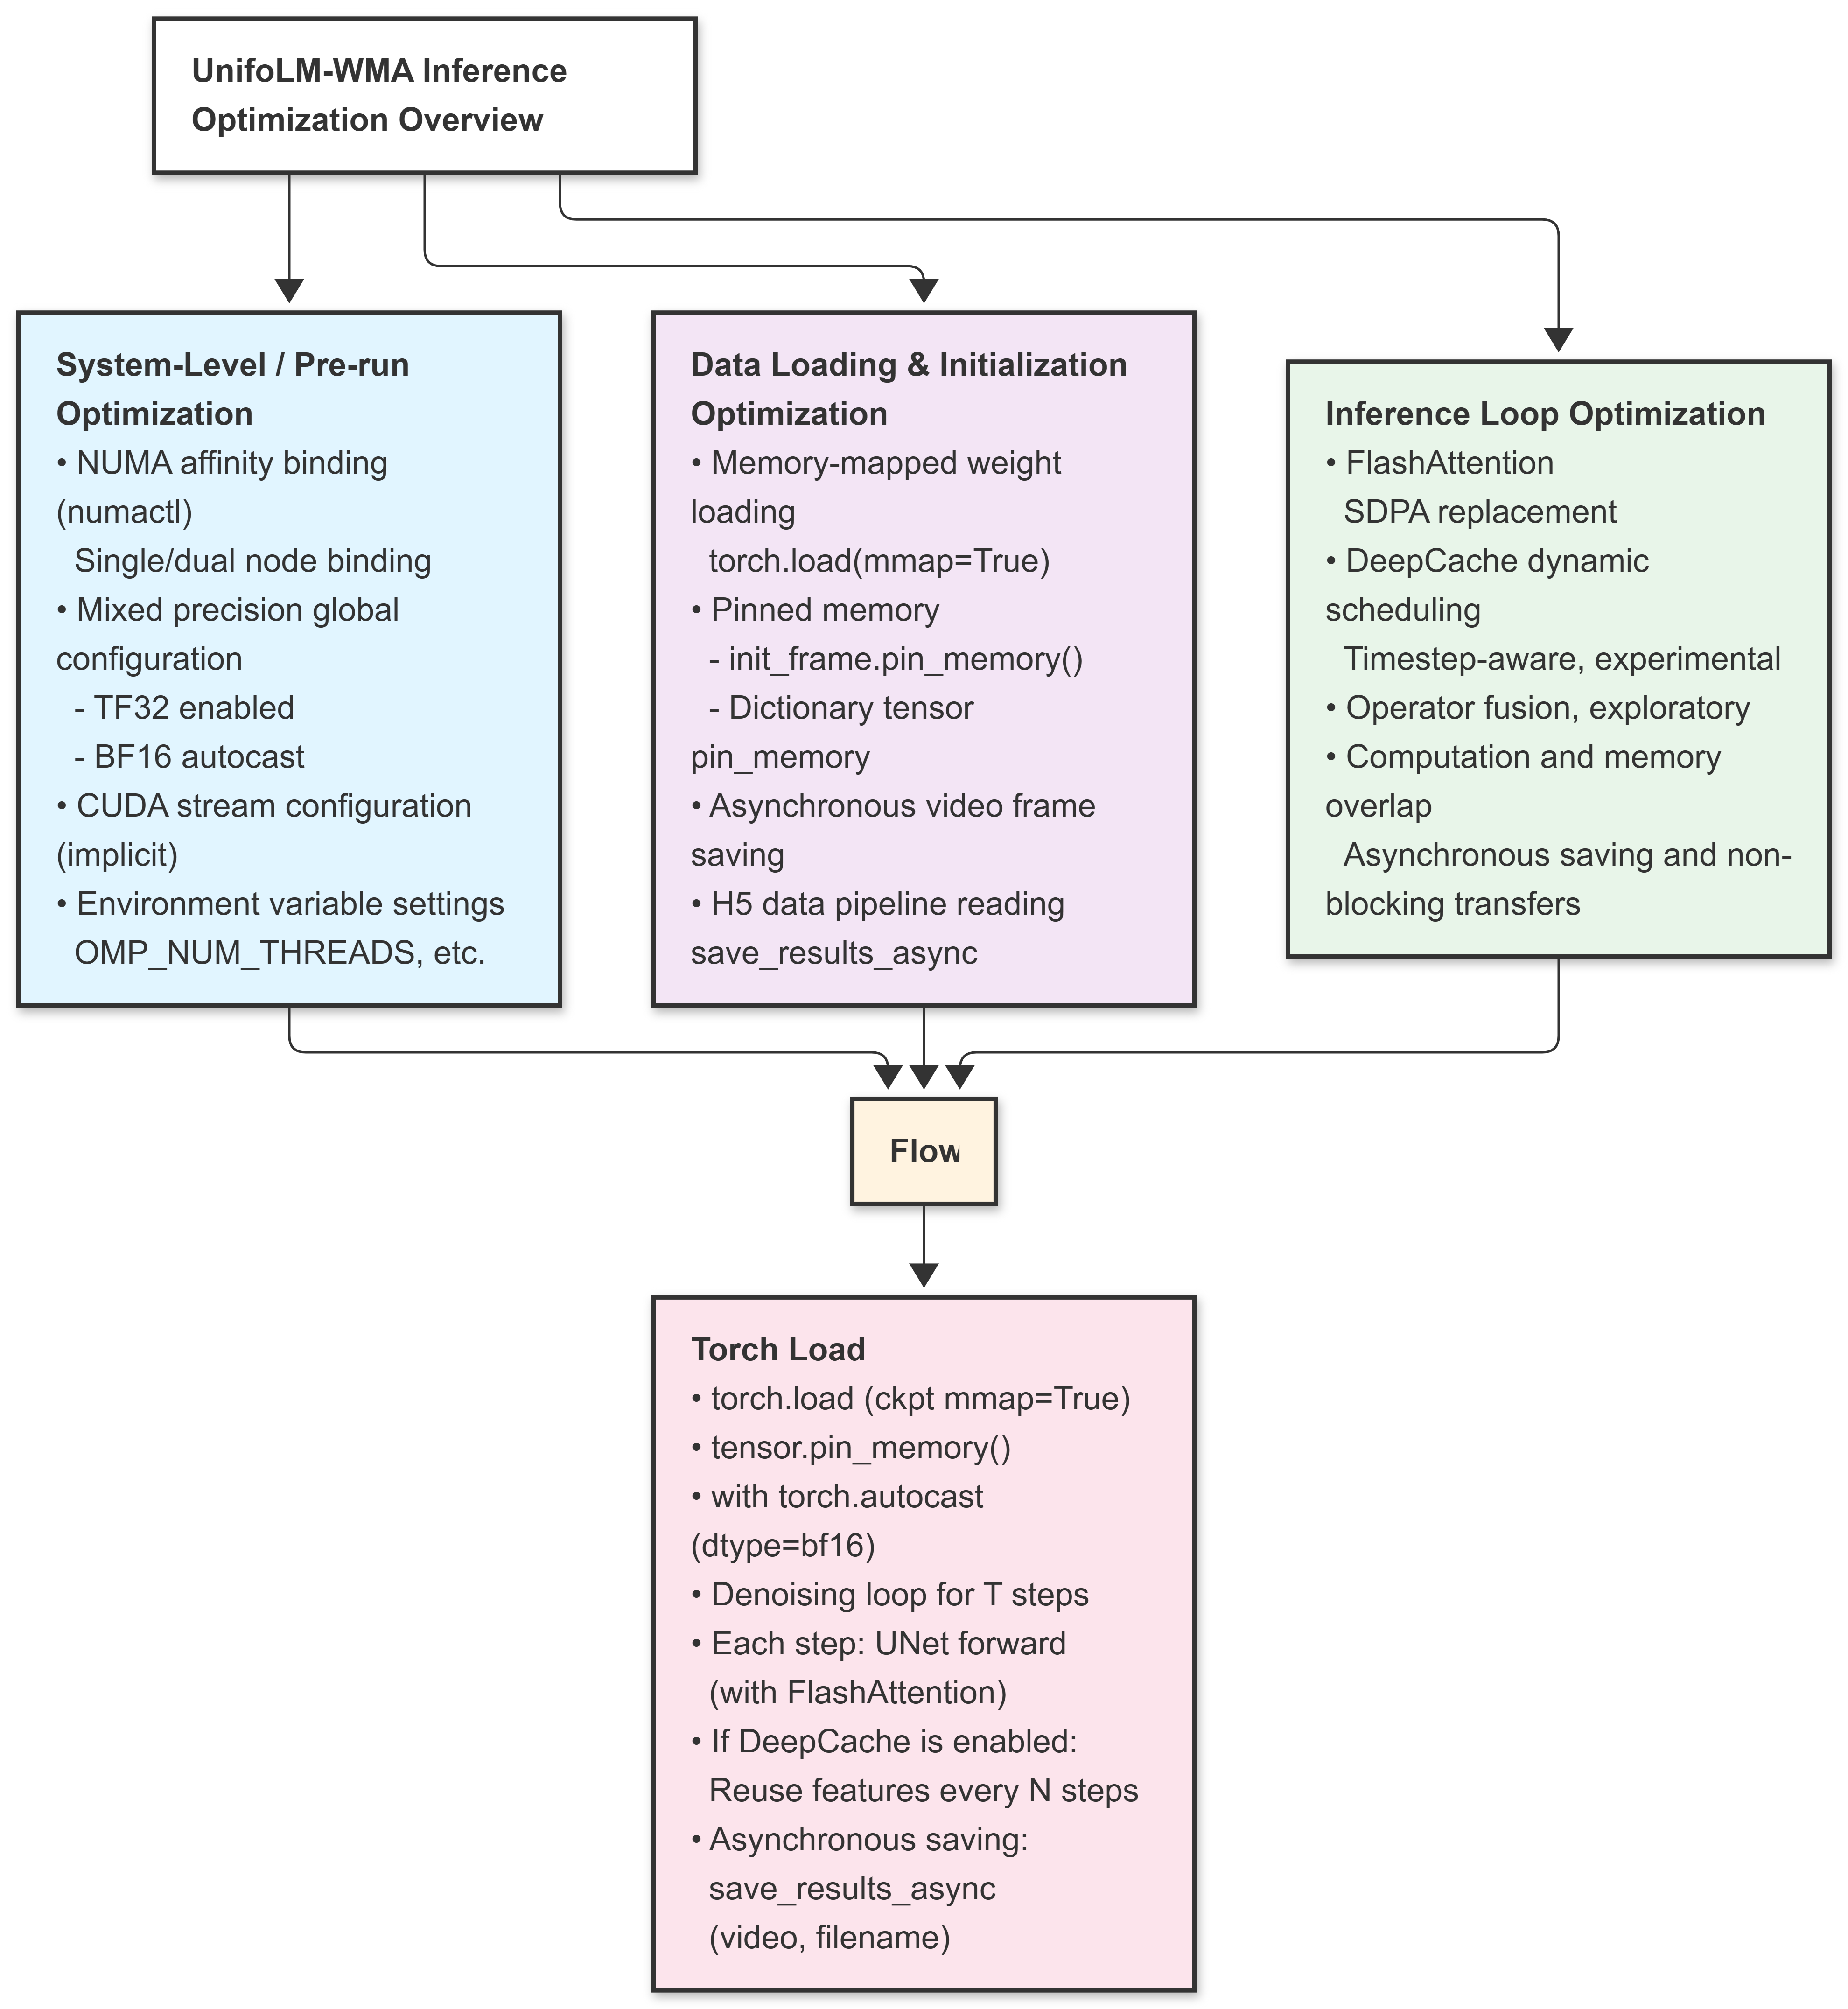
\includegraphics[width=0.8\linewidth]{Br_ Memory Flow-2026-03-02-102603.png}
    \caption{Workflow Optimization Map}
    \label{fig:unifo overview}
\end{figure}


To systematically enhance the inference efficiency of UnifoLM-WMA, we designed a collaborative optimization scheme across three levels, as illustrated in Figure \ref{fig:unifo overview}.

(1) System-Level Pre-configuration

Prior to model execution, NUMA affinity is enforced using the numactl tool to ensure that CPU memory accesses and GPU resources are confined to the same physical node, thereby eliminating latency overhead incurred by cross-node communication. 
Concurrently, global mixed-precision settings are enabled: TF32 format is permitted to accelerate matrix operations, while BF16 automatic mixed precision (autocast) is applied in core computational regions to reduce memory footprint and data transfer volume.

(2) Data Loading and I/O Optimization

To address bottlenecks associated with loading large-scale model weights and input data, we employ memory-mapped loading via torch.load(mmap=True), eliminating redundant CPU memory copies. Input images and tensors are pinned to page-locked memory using .pin memory() to accelerate CPU-to-GPU transfer efficiency. For H5-format input data, a pipelined reading mechanism is constructed to minimize I/O waiting. For video frame saving, an asynchronous saving function save results async is designed to offload post-processing and disk write operations to background threads, allowing the main thread to proceed directly to the next inference iteration.

(3) Inference Loop Optimization

Within the core denoising loop, FlashAttention replaces standard attention implementations to reduce memory read/write overhead. The DeepCache scheduling strategy remains under experimental investigation to determine optimal parameter configurations: through a timestep-aware caching mechanism, deep features are reused every N steps, bypassing full U-Net forward passes and thereby reducing computational load. Computation and storage overlap is achieved through asynchronous saving and non-blocking transfers, ensuring sustained GPU computation during I/O operations. Operator fusion is currently in the exploratory phase and is considered a direction for future optimization.

Overall Data Flow: After model weights are loaded via memory mapping, input data is transferred to the GPU through pinned memory. Within the BF16 automatic mixed-precision context, a T-step denoising loop is executed, where each U-Net forward pass integrates FlashAttention; if DeepCache is enabled, features are reused at set intervals. The generated video is ultimately saved to disk via the asynchronous function, achieving substantial overlap between computation and I/O.

%todo：overview的图和说明。
% 在 6.2 部分


\subsubsection{NUMA Affinity Optimization}
\

\begin{comment}
从 NUMA 架构的角度来看，服务器 A 是单 node 结构，服务器 B 是双 node 架构. 该优化方法针对以服务器 B 为代表的多 node NUMA 架构机器.

我们通过使用 numactl 工具将脚本的运行和 CPU 调度，GPU 使用都在同一个 node 节点上进行，避免跨 node 节点访问，预计提速 10% 左右.

在双路 NUMA 架构中，CPU、内存与 GPU 被物理分割在两个独立的节点（Socket）中。当计算进程运行在一个节点，却需要调用另一个节点的内存或 GPU 时，
数据必须跨越节点间总线（如 QPI/UPI）。这种跨节点访问会引入较高的延迟，并受限于总线带宽上限，在大规模推理任务中极易引发数据拥塞，成为性能瓶颈。、
使用 numactl 工具可以建立“硬件局部性（Hardware Locality）”。通过操作系统调度，强制将计算进程、物理内存和目标 GPU 锁定在同一个物理节点内。
这种方式确保了任务与其所需资源在物理拓扑上完全对齐，消除了跨节点通信产生的多余开销，从而显著提升系统的整体吞吐量，提高模型推理速度.\textbf{}

Server B Baseline Test Results
Server B Taking NUMA Affinity Optimization's Results
NUMA Affinity OPtimization's performance
\end{comment}

\begin{table}[!htbp]
    \centering
    \small
    \renewcommand{\arraystretch}{1.0}
    \caption{Impact of NUMA Affinity Optimization on Server B Inference,where the baseline performance is detailed in Section \ref{sec:unif exp reult}. And, the values in the parentheses of the ``Test Time" and ``Test PSNR" columns respectively represent the speedup ratio relative to the baseline time and the difference to baseline PSNR.}
    \label{tab:server_b_numa}
    \begin{tabular}{|>{\centering\arraybackslash}m{6cm}|c|c|c|}
        \hline
        \rowcolor{yellow} \textbf{Scenario} & \textbf{Case} & \textbf{Test Time} & \textbf{Test PSNR} \\ \hline
        
        \multirow{4}{*}{unitree\_g1\_pack\_camera} 
        & 1 & 19m26.800s / 1166.800 s (1.230$\times$)& 18.5229(0) \\ \cline{2-4}
        & 2 & 19m25.073s / 1165.073 s(1.236$\times$) & 18.5432(0)\\ \cline{2-4}
        & 3 & 19m20.739s / 1160.739 s(1.241$\times$)& 19.9578(0) \\ \cline{2-4}
        & 4 & 19m22.388s / 1162.388 s(1.236$\times$) & 17.7746(0)\\ \hline
        
        \multirow{4}{*}{unitree\_z1\_stackbox}     
        & 1 & 20m54.452s / 1254.452 s(1.238 $\times$) & 23.9826(0)\\ \cline{2-4}
        & 2 & 20m53.071s / 1253.071 s(1.243$\times$) & 20.0572(0)\\ \cline{2-4}
        & 3 & 20m53.853s / 1253.853 s(1.240$\times$) & 21.7059(0)\\ \cline{2-4}
        & 4 & 20m52.502s / 1252.502 s(1.243 $\times$) & 25.2775(0)\\ \hline
        
        \multirow{4}{*}{unitree\_z1\_dual\_arm\_stackbox\_v2} 
        & 1 & 19m33.918s / 1173.918 s(1.234$\times$) & 20.0181(0)\\ \cline{2-4}
        & 2 & 19m29.337s / 1169.337 s(1.238$\times$) & 18.8915(0)\\ \cline{2-4}
        & 3 & 19m32.557s / 1172.557 s(1.236$\times$) & 18.8271(0)\\ \cline{2-4}
        & 4 & 19m31.043s / 1171.043 s(1.237 $\times$) & 19.3431(0)\\ \hline
        
        \multirow{4}{*}{unitree\_z1\_dual\_arm\_stackbox}     
        & 1 & 13m5.162s / 785.162 s (1.226$\times$)& 22.8169(0)\\ \cline{2-4}
        & 2 & 13m5.668s / 785.668 s (1.229$\times$)& 24.5789(0)\\ \cline{2-4}
        & 3 & 13m5.123s / 785.123 s (1.225$\times$)& 26.2675(0)\\ \cline{2-4}
        & 4 & 13m4.947s / 784.947 s (1.228$\times$)& 25.3952(0)\\ \hline
        
        \multirow{4}{*}{unitree\_z1\_dual\_arm\_cleanup\_pencils} 
        & 1 & 14m31.863s / 871.863 s(1.231$\times$) & 21.2321(0)\\ \cline{2-4}
        & 2 & 14m32.574s / 872.574 s(1.234$\times$)& 22.5411(0)\\ \cline{2-4}
        & 3 & 14m33.037s / 873.037 s(1.229$\times$) & 19.9960(0)\\ \  cline{2-4}
        & 4 & 14m32.806s / 872.806 s(1.234$\times$) & 22.8648(0)\\ \hline
        \textbf{Average}&-& 17m45.346s / 1065.346s(1.234$\times$)&21.4297(0) \\ \hline
    \end{tabular}
\end{table}

From the perspective of Non-Uniform Memory Access (NUMA) topology, ``Server A" features a single-node structure, whereas ``Server B" employs a dual-node architecture. 
The optimization strategy detailed herein is specifically designed for multi-node NUMA systems, as exemplified by ``Server B".

In a dual-socket NUMA configuration, CPUs, memory, and GPUs are physically partitioned across distinct hardware nodes (sockets).
Consequently, when a computational process residing on one node attempts to access memory or GPU resources located on the other, the data must traverse the interconnect bus (e.g., QuickPath Interconnect or UltraPath Interconnect). 
This cross-node communication introduces substantial latency and is strictly constrained by the bandwidth limits of the bus. 
During intensive, large-scale inference tasks, such architectural constraints frequently induce data congestion, manifesting as a critical performance bottleneck.

To mitigate this bottleneck, we utilize the numactl utility to enforce strict hardware locality. 
By leveraging OS-level scheduling, this approach confines script execution, CPU scheduling, memory allocation, and target GPU utilization entirely within a single physical node. 
This strategy guarantees a precise topological alignment between computational tasks and their requisite hardware resources. 
By circumventing the redundant overhead associated with cross-node communication, this method substantially enhances the overall system throughput and accelerates model inference, \textbf{resulting in an approximately 23.4\% reduction in inference time as shown in Table \ref{tab:server_b_numa}(the baseline test on ``Server B" is shown in Table \ref{tab:server_b_baseline}).} Since NUMA binding operates strictly as an OS-level optimization for hardware resource scheduling, it does not interfere with the model's underlying mathematical logic. \textbf{Consequently, the PSNR of the generated videos remains unaffected, yielding a mean variance of zero.}



%caption第一个表格解释了，后续就不再赘述；PSNR的变化平均值没写。
% done



% \begin{table}[!htbp]
%     \centering
%     \renewcommand{\arraystretch}{1.0}
%     \caption{Detailed Efficiency Analysis of NUMA Affinity Optimization on Server B}
%     \label{tab:numa_eval}
%     \begin{tabular}{|>{\centering\arraybackslash}m{5.8cm}|c|c|c|}
%         \hline
%         \rowcolor{yellow} \textbf{Scenario} & \textbf{Case} & \textbf{Diff Time} & \textbf{Speedup} \\ \hline
        
%         \multirow{4}{*}{unitree\_g1\_pack\_camera} 
%         & 1 & \textcolor{diffgreen}{\textbf{-268.242}} & 1.230 \\ \cline{2-4}
%         & 2 & \textcolor{diffgreen}{\textbf{-275.394}} & 1.236 \\ \cline{2-4}
%         & 3 & \textcolor{diffgreen}{\textbf{-279.310}} & 1.241 \\ \cline{2-4}
%         & 4 & \textcolor{diffgreen}{\textbf{-274.493}} & 1.236 \\ \hline
        
%         \multirow{4}{*}{unitree\_z1\_stackbox}     
%         & 1 & \textcolor{diffgreen}{\textbf{-298.783}} & 1.238 \\ \cline{2-4}
%         & 2 & \textcolor{diffgreen}{\textbf{-304.013}} & 1.243 \\ \cline{2-4}
%         & 3 & \textcolor{diffgreen}{\textbf{-300.515}} & 1.240 \\ \cline{2-4}
%         & 4 & \textcolor{diffgreen}{\textbf{-304.661}} & 1.243 \\ \hline
        
%         \multirow{4}{*}{unitree\_z1\_dual\_arm\_stackbox\_v2} 
%         & 1 & \textcolor{diffgreen}{\textbf{-274.348}} & 1.234 \\ \cline{2-4}
%         & 2 & \textcolor{diffgreen}{\textbf{-278.736}} & 1.238 \\ \cline{2-4}
%         & 3 & \textcolor{diffgreen}{\textbf{-277.114}} & 1.236 \\ \cline{2-4}
%         & 4 & \textcolor{diffgreen}{\textbf{-277.036}} & 1.237 \\ \hline
        
%         \multirow{4}{*}{unitree\_z1\_dual\_arm\_stackbox}     
%         & 1 & \textcolor{diffgreen}{\textbf{-177.274}} & 1.226 \\ \cline{2-4}
%         & 2 & \textcolor{diffgreen}{\textbf{-180.053}} & 1.229 \\ \cline{2-4}
%         & 3 & \textcolor{diffgreen}{\textbf{-176.711}} & 1.225 \\ \cline{2-4}
%         & 4 & \textcolor{diffgreen}{\textbf{-179.074}} & 1.228 \\ \hline
        
%         \multirow{4}{*}{unitree\_z1\_dual\_arm\_cleanup\_pencils} 
%         & 1 & \textcolor{diffgreen}{\textbf{-201.198}} & 1.231 \\ \cline{2-4}
%         & 2 & \textcolor{diffgreen}{\textbf{-204.318}} & 1.234 \\ \cline{2-4}
%         & 3 & \textcolor{diffgreen}{\textbf{-199.552}} & 1.229 \\ \cline{2-4}
%         & 4 & \textcolor{diffgreen}{\textbf{-204.002}} & 1.234 \\ \hline
%     \end{tabular}
% \end{table}




\subsubsection{Mixed Precision}
\

\begin{comment}
混合精度优化的基本原理在于，深度神经网络对数值的微小误差并不敏感，不需要极高的小数精度也能保持输出结果的准确。
在模型推理时，将常规的 32 位浮点数（FP32）替换为 16 位的 BF16 或 TF32 格式，最直接的效果是将模型参数和计算时产生的数据总量缩减了一半。
数据变小后，系统在内存和 GPU 之间搬运数据的负担大幅减轻，直接缓解了数据传输慢导致的 I/O 堵塞问题，也提高了数据传输的速度。 
BF16 通过截断尾数保留了与 FP32 相同的指数位宽（即维持了数值的动态范围），而 TF32 则在内部计算时利用了低位宽乘法的硬件优势。
同时，由于单笔计算的数据变短了，现代 GPU 内部的计算单元可以在同一个时钟周期内并行处理更多的浮点运算，让现有的计算资源发挥出成倍的吞吐量。
简而言之，混合精度通过合理舍弃多余的小数精度，换取了更小的显存占用和更快的数据流转，
在确保生成视频质量（PSNR）损失较低的情况下，切实提升整体的推理速度。

在具体优化上，可以分为 3 个可选的独立部分：

一是在全局计算后端的环境配置中，通过置位 torch.backends.cuda.matmul.allow_tf32 = True 
与 torch.backends.cudnn.allow_tf32 = True 开启硬件级的 TF32（TensorFloat-32）加速机制。该指令允许 CUDA 和 cuDNN 核心库在执行矩阵乘法和卷积操作时，
自动将输入的 FP32 数据无缝转换为 TF32 格式。TF32 格式巧妙地截取了 FP32 的 8 位指数域以保证同样的动态范围防止溢出，同时保留了 FP16 的 10 位尾数域以满足模型所需的精度。

二是在核心的扩散去噪循环（如动作序列向量生成，视频序列帧生成）中引入了基于 bfloat16 的自动混合精度（AMP）推理架构。通过使用 torch.autocast(device_type="cuda", dtype=torch.bfloat16) 上下文管理器，
构建一个智能的精度调度机制。该机制能够动态识别计算图中的算子特征：针对计算密集型算子（如 Linear、Conv2d），其输入会被自动转换为 bfloat16 并送入 Tensor Core 极速计算；
而对于对数值精度极度敏感的算子（如 LayerNorm、Softmax），则严格保留 FP32 格式以维持数值稳定性。

三是对 unifolm_wma_dual.ckpt 和 ViT-H-14 模型的权重进行短精度截断再从 CPU 内存移进显存，实现 PCIe 总线在传输模型权重时数据运输压力减半.

在服务器 A 上，我们尝试过同时采取上述 3 个措施进行混合精度优化，但发现会有部分 case 的 psnr 值不达标，于是在服务器 A 上，我们选择了保守的混合精度优化方案，
只采取前面两种措施（且不在世界模型生成视频序列帧的推理循环中启用混合精度）。采用该优化方法后，平均每个 case 的加速比为 1.33X，具体优化效果如下：

对于服务器 B，我们采取了激进的混合精度优化方案，同时采取上述所有优化措施，具体结果如下：

请专业，学术，简要，优雅地将这段话整理成英文材料
\end{comment}
The fundamental principle of mixed-precision optimization relies on the fact that deep neural networks are generally insensitive to minor numerical variances, allowing them to maintain output accuracy without requiring extremely high decimal precision. 
During model inference, replacing standard 32-bit floating-point (FP32) formats with 16-bit BF16 or TF32 (TensorFloat-32) formats directly halves the total data volume of model parameters and intermediate computations. 
This reduction significantly alleviates the data transfer payload between system memory and the GPU, effectively mitigating I/O bottlenecks and accelerating transmission speeds. 
Specifically, BF16 retains the same exponent width as FP32 by truncating the mantissa, thereby preserving the dynamic range; meanwhile, TF32 leverages hardware-level advantages for low bit-width multiplication during internal computations.  
Furthermore, because the individual data elements are shorter, modern GPU computing units can process a greater number of floating-point operations in parallel within a single clock cycle, multiplicatively increasing the throughput of existing hardware. 
In summary, mixed precision trades unnecessary decimal precision for a smaller memory footprint and faster data flow, tangibly improving overall inference speed while ensuring minimal degradation in the generated video quality (PSNR).

%表信息修改
\begin{table}[!htbp]
    \centering
    \small
    \renewcommand{\arraystretch}{1.0}
    \caption{Impact of Mixed Precision Optimization on Server A Inference, where the baseline performance is detailed in Section \ref{sec:unif exp reult}.}
    \label{tab:server_b_precision2}
    \begin{tabular}{|>{\centering\arraybackslash}m{6cm}|c|c|c|}
        \hline
        \rowcolor{yellow} \textbf{Scenario} & \textbf{Case} & \textbf{Test Time} & \textbf{Test PSNR} \\ \hline
        
        \multirow{4}{*}{unitree\_g1\_pack\_camera} 
        & 1 & 9m29.502s / 569.502 s (1.297$\times$) & 36.2602(0.619) \\ \cline{2-4}
        & 2 & 7m43.190s / 463.190 s (1.357$\times$) & 42.7647(9.462) \\ \cline{2-4}
        & 3 & 7m50.046s / 470.046 s (1.333$\times$) & 34.4601(-4.614) \\ \cline{2-4}
        & 4 & 7m41.468s / 461.468 s (1.365$\times$) & 33.5926(-0.535) \\ \hline
        
        \multirow{4}{*}{unitree\_z1\_stackbox}     
        & 1 & 8m13.019s / 493.019 s (1.387$\times$) & 48.3723(-0.542) \\ \cline{2-4}
        & 2 & 8m15.012s / 495.012 s (1.377$\times$) & 47.5901(6.848) \\ \cline{2-4}
        & 3 & 8m14.072s / 494.072 s (1.363$\times$) & 48.0674(-1.713) \\ \cline{2-4}
        & 4 & 8m18.593s / 498.593 s (1.364$\times$) & 47.1862(-0.075) \\ \hline
        
        \multirow{4}{*}{unitree\_z1\_dual\_arm\_stackbox\_v2} 
        & 1 & 7m48.821s / 468.821 s (1.355$\times$) & 25.2486(-0.819) \\ \cline{2-4}
        & 2 & 7m45.663s / 465.663 s (1.365$\times$) & 27.1028(-3.405) \\ \cline{2-4}
        & 3 & 8m3.851s / 483.851 s (1.326$\times$) & 32.4244(0.431) \\ \cline{2-4}
        & 4 & 7m52.203s / 472.203 s (1.351$\times$) & 34.2318(-4.998) \\ \hline
        
        \multirow{4}{*}{unitree\_z1\_dual\_arm\_stackbox}     
        & 1 & 5m32.981s / 332.981 s (1.307$\times$) & 43.8239(4.693) \\ \cline{2-4}
        & 2 & 5m32.647s / 332.647 s (1.307$\times$) & 42.1073(2.184) \\ \cline{2-4}
        & 3 & 5m33.863s / 333.863 s (1.312$\times$) & 36.0992(-0.586) \\ \cline{2-4}
        & 4 & 5m33.525s / 333.525 s (1.308$\times$) & 47.0527(5.542) \\ \hline
        
        \multirow{4}{*}{unitree\_z1\_dual\_arm\_cleanup\_pencils} 
        & 1 & 5m57.565s / 357.565 s (1.348$\times$) & 45.5420(2.243) \\ \cline{2-4}
        & 2 & 5m59.465s / 359.465 s (1.344$\times$) & 47.2762(-1.403) \\ \cline{2-4}
        & 3 & 5m58.024s / 358.024 s (1.345$\times$) & 47.1712(5.012) \\ \cline{2-4}
        & 4 & 5m59.335s / 359.335 s (1.334$\times$) & 46.5297(0.124) \\ \hline
        
        \textbf{Average} & - & 7m10.142s / 430.142 s (1.342$\times$) & 40.6452 (0.9232)\\ \hline
    \end{tabular}
\end{table}

%表信息修改;表引用与说明
\begin{table}[!htbp]
    \centering
    \small
    \renewcommand{\arraystretch}{1.0}
    \caption{Impact of Mixed Precision Optimization improved on Server B Inference, where the baseline performance is detailed in Section \ref{sec:unif exp reult}. }
    \label{tab:server_b_mixec_precision}
    \begin{tabular}{|>{\centering\arraybackslash}m{6cm}|c|c|c|}
        \hline
        \rowcolor{yellow} \textbf{Scenario} & \textbf{Case} & \textbf{Test Time} & \textbf{Test PSNR} \\ \hline
        
        \multirow{4}{*}{unitree\_g1\_pack\_camera} 
        & 1 & 10m58.948s / 658.948 s (2.178$\times$) & 18.707(0.180) \\ \cline{2-4}
        & 2 & 10m58.109s / 658.109 s (2.189$\times$) & 18.708(0.170) \\ \cline{2-4}
        & 3 & 10m57.763s / 657.763 s (2.189$\times$) & 19.662(0.300) \\ \cline{2-4}
        & 4 & 10m58.393s / 658.393 s (2.182$\times$) & 17.512(-0.260) \\ \hline
        
        \multirow{4}{*}{unitree\_z1\_stackbox}     
        & 1 & 11m45.120s / 705.120 s (2.203$\times$) & 24.146(0.160) \\ \cline{2-4}
        & 2 & 11m46.028s / 706.028 s (2.205$\times$) & 20.153(0.100) \\ \cline{2-4}
        & 3 & 11m45.068s / 705.068 s (2.205$\times$) & 21.766(0.060) \\ \cline{2-4}
        & 4 & 11m41.959s / 701.959 s (2.218$\times$) & 23.450(-1.830) \\ \hline
        
        \multirow{4}{*}{unitree\_z1\_dual\_arm\_stackbox\_v2} 
        & 1 & 11m8.558s / 668.558 s (2.166$\times$) & 19.174(-0.840) \\ \cline{2-4}
        & 2 & 11m7.047s / 667.047 s (2.171$\times$) & 19.730(0.840) \\ \cline{2-4}
        & 3 & 11m9.955s / 669.955 s (2.164$\times$) & 19.836(1.010) \\ \cline{2-4}
        & 4 & 11m13.538s / 673.538 s (2.150$\times$) & 19.515(0.170) \\ \hline
        
        \multirow{4}{*}{unitree\_z1\_dual\_arm\_stackbox}     
        & 1 & 7m50.265s / 470.265 s (2.047$\times$) & 23.716(0.900) \\ \cline{2-4}
        & 2 & 7m45.591s / 465.591 s (2.074$\times$) & 25.844(1.270) \\ \cline{2-4}
        & 3 & 7m45.791s / 465.791 s (2.065$\times$) & 25.235(1.030) \\ \cline{2-4}
        & 4 & 7m50.022s / 470.022 s (2.051$\times$) & 25.368(0.030) \\ \hline
        
        \multirow{4}{*}{unitree\_z1\_dual\_arm\_cleanup\_pencils} 
        & 1 & 8m27.712s / 507.712 s (2.114$\times$) & 20.366(-0.870) \\ \cline{2-4}
        & 2 & 8m32.725s / 512.725 s (2.100$\times$) & 20.033(-2.510) \\ \cline{2-4}
        & 3 & 8m28.134s / 508.134 s (2.111$\times$) & 20.235(0.240) \\ \cline{2-4}
        & 4 & 8m26.754s / 506.754 s (2.125$\times$) & 22.741(0.120) \\ \hline
        
        \textbf{Average} & - & 10m1.874s / 601.874 s (2.145$\times$) & 21.295 (-0.1327)\\ \hline
    \end{tabular}
\end{table}

Regarding specific implementation, this optimization can be divided into three independent optional components. 
\begin{enumerate}%TF32，FP32，BF16等描述的一致性和正确使用（缩写只需要在第一次出现的时候把全称写出来）。
    \item First, at the global backend configuration level, we enable hardware-level TF32 acceleration \textbf{torch.backends.cuda.matmul.allow\_tf32 = True} and \textbf{torch.backends.cudnn.allow\_tf32 = True}. 
    These directives allow the CUDA and cuDNN core libraries to automatically convert input FP32 data into the TF32 format during matrix multiplications and convolutions. 
    The TF32 format utilizes an 8-bit exponent to maintain the same dynamic range as FP32 to prevent overflow, while retaining a 10-bit mantissa to satisfy the model's precision requirements.
    \item Second, we introduce a BF16-based Automatic Mixed Precision (AMP) inference architecture within the core diffusion denoising loops, such as action sequence vector generation and video sequence frame generation. 
    By utilizing the \textbf{torch.autocast(device\_type``cuda'', dtype=torch.bfloat16)} context manager, we establish an intelligent precision scheduling mechanism. 
    This mechanism dynamically identifies operator characteristics within the computational graph: inputs for compute-intensive operators (e.g., Linear, Conv2d) are automatically converted to BF16 and routed to Tensor Cores for rapid computation, whereas precision-sensitive operators (e.g., LayerNorm, Softmax) are strictly preserved in FP32 to ensure numerical stability.
    \item Third, we perform precision truncation on the weights of the \textbf{unifolm\_wma\_dual.ckpt} and \textbf{ViT-H-14} models before transferring them from CPU memory to the GPU. 
    This strategy effectively halves the data transmission pressure on the PCIe(Peripheral Component Interconnect Express) bus during model weight loading.
\end{enumerate}


On Server A, we initially attempted to apply all three mixed-precision measures simultaneously. 
However, we observed that the PSNR values for certain test cases failed to meet the required threshold. 
Consequently, we adopted a conservative mixed-precision optimization strategy for Server A, implementing only the first two measures and explicitly disabling AMP within the world model's video sequence frame generation loop. 
\textbf{This optimization delivered an average per-case speedup of 1.342$\times$.} 
The specific optimization results are as shown in Table \ref{tab:server_b_precision2}.% server B三种的效果也呈现一下；加上修改后Table的引用。

For Server B, we employed an aggressive mixed-precision strategy, applying all three optimization measures simultaneously. 
\textbf{The specific results are detailed  in Table \ref{tab:server_b_mixec_precision} with  an average per-case speedup of 2.145$\times$.}

As mixed precision is adopted, where the numerical precision of bf16 and tf32 is lower than that of float32 which is used by unifolm-wma as the original precision, inferences with mixed precision on Both Server A and Server B lead to a decrease in PSNR values for some cases.



% \begin{table}[!htbp]
%     \centering
%     \renewcommand{\arraystretch}{1.0}
%     \caption{PSNR Performance Profiling under Mixed Precision Strategy on Server A}
%     \label{tab:Precision2_PSNR对比}
%     \begin{tabular}{|>{\centering\arraybackslash}m{5.8cm}|c|c|c|}
%         \hline
%         \rowcolor{yellow} \textbf{Scenario} & \textbf{Case} & \textbf{Baseline PSNR} & \textbf{Test PSNR} \\
%         \hline
%         \multirow{4}{*}{unitree\_g1\_pack\_camera} & 1 & 35.641 & 35.641 \\
%         \cline{2-4}
%         & 2 & 33.303 & 33.303 \\
%         \cline{2-4}
%         & 3 & 39.074 & 39.074 \\
%         \cline{2-4}
%         & 4 & 34.128 & 34.128 \\
%         \hline
%         \multirow{4}{*}{unitree\_z1\_stackbox} & 1 & 48.914 & 48.914 \\
%         \cline{2-4}
%         & 2 & 40.743 & 40.743 \\
%         \cline{2-4}
%         & 3 & 49.781 & 49.781 \\
%         \cline{2-4}
%         & 4 & 47.261 & 47.261 \\
%         \hline
%         \multirow{4}{*}{unitree\_z1\_dual\_arm\_stackbox\_v2} & 1 & 26.068 & 26.068 \\
%         \cline{2-4}
%         & 2 & 30.508 & 30.508 \\
%         \cline{2-4}
%         & 3 & 31.994 & 31.994 \\
%         \cline{2-4}
%         & 4 & 39.229 & 39.229 \\
%         \hline
%         \multirow{4}{*}{unitree\_z1\_dual\_arm\_stackbox} & 1 & 39.131 & 39.131 \\
%         \cline{2-4}
%         & 2 & 39.923 & 39.923 \\
%         \cline{2-4}
%         & 3 & 36.685 & 36.685 \\
%         \cline{2-4}
%         & 4 & 41.511 & 41.511 \\
%         \hline
%         \multirow{4}{*}{unitree\_z1\_dual\_arm\_cleanup\_pencils} & 1 & 43.299 & 43.299 \\
%         \cline{2-4}
%         & 2 & 48.679 & 48.679 \\
%         \cline{2-4}
%         & 3 & 42.159 & 42.159 \\
%         \cline{2-4}
%         & 4 & 46.405 & 46.405 \\
%         \hline
%     \end{tabular}
% \end{table}

% \begin{table}[!htbp]
%     \centering
%     \renewcommand{\arraystretch}{1.0}
%     \caption{Inference Latency Assessment: Acceleration Gains via Mixed Precision Optimization on Server A}
%     \label{tab:Precision2_时间差异与速度}
%     \begin{tabular}{|>{\centering\arraybackslash}m{5.8cm}|c|c|c|}
%         \hline
%         \rowcolor{yellow} \textbf{Scenario} & \textbf{Case} & \textbf{Diff Time} & \textbf{Velocity} \\
%         \hline
%         \multirow{4}{*}{unitree\_g1\_pack\_camera} & 1 & \textcolor{diffgreen}{\textbf{-169.084}} & 1.30X \\
%         \cline{2-4}
%         & 2 & \textcolor{diffgreen}{\textbf{-165.381}} & 1.36X \\
%         \cline{2-4}
%         & 3 & \textcolor{diffgreen}{\textbf{-156.318}} & 1.33X \\
%         \cline{2-4}
%         & 4 & \textcolor{diffgreen}{\textbf{-168.599}} & 1.37X \\
%         \hline
%         \multirow{4}{*}{unitree\_z1\_stackbox} & 1 & \textcolor{diffgreen}{\textbf{-190.729}} & 1.39X \\
%         \cline{2-4}
%         & 2 & \textcolor{diffgreen}{\textbf{-186.387}} & 1.38X \\
%         \cline{2-4}
%         & 3 & \textcolor{diffgreen}{\textbf{-179.330}} & 1.36X \\
%         \cline{2-4}
%         & 4 & \textcolor{diffgreen}{\textbf{-181.321}} & 1.36X \\
%         \hline
%         \multirow{4}{*}{unitree\_z1\_dual\_arm\_stackbox\_v2} & 1 & \textcolor{diffgreen}{\textbf{-166.658}} & 1.36X \\
%         \cline{2-4}
%         & 2 & \textcolor{diffgreen}{\textbf{-170.000}} & 1.37X \\
%         \cline{2-4}
%         & 3 & \textcolor{diffgreen}{\textbf{-157.827}} & 1.33X \\
%         \cline{2-4}
%         & 4 & \textcolor{diffgreen}{\textbf{-165.583}} & 1.35X \\
%         \hline
%         \multirow{4}{*}{unitree\_z1\_dual\_arm\_stackbox} & 1 & \textcolor{diffgreen}{\textbf{-102.199}} & 1.31X \\
%         \cline{2-4}
%         & 2 & \textcolor{diffgreen}{\textbf{-102.261}} & 1.31X \\
%         \cline{2-4}
%         & 3 & \textcolor{diffgreen}{\textbf{-104.088}} & 1.31X \\
%         \cline{2-4}
%         & 4 & \textcolor{diffgreen}{\textbf{-102.714}} & 1.31X \\
%         \hline
%         \multirow{4}{*}{unitree\_z1\_dual\_arm\_cleanup\_pencils} & 1 & \textcolor{diffgreen}{\textbf{-124.497}} & 1.35X \\
%         \cline{2-4}
%         & 2 & \textcolor{diffgreen}{\textbf{-123.690}} & 1.34X \\
%         \cline{2-4}
%         & 3 & \textcolor{diffgreen}{\textbf{-123.678}} & 1.35X \\
%         \cline{2-4}
%         & 4 & \textcolor{diffgreen}{\textbf{-120.029}} & 1.33X \\
%         \hline
%     \end{tabular}
% \end{table}




% \begin{table}[!htbp]
%     \centering
%     \renewcommand{\arraystretch}{1.0}
%     \caption{Inference Latency Assessment: Acceleration Gains via Mixed Precision Optimization on Server B}
%     \label{tab:method2_改良_时间差异与速度}
%     \begin{tabular}{|>{\centering\arraybackslash}m{5.8cm}|c|c|c|}
%         \hline
%         \rowcolor{yellow} \textbf{Scenario} & \textbf{Case} & \textbf{Diff Time} & \textbf{Velocity} \\
%         \hline
%         \multirow{4}{*}{unitree\_g1\_pack\_camera} & 1 & \textcolor{diffgreen}{\textbf{-776.094}} & 2.18X \\
%         \cline{2-4}
%         & 2 & \textcolor{diffgreen}{\textbf{-782.358}} & 2.19X \\
%         \cline{2-4}
%         & 3 & \textcolor{diffgreen}{\textbf{-782.286}} & 2.19X \\
%         \cline{2-4}
%         & 4 & \textcolor{diffgreen}{\textbf{-778.488}} & 2.18X \\
%         \hline
%         \multirow{4}{*}{unitree\_z1\_stackbox} & 1 & \textcolor{diffgreen}{\textbf{-848.115}} & 2.20X \\
%         \cline{2-4}
%         & 2 & \textcolor{diffgreen}{\textbf{-851.056}} & 2.21X \\
%         \cline{2-4}
%         & 3 & \textcolor{diffgreen}{\textbf{-849.300}} & 2.20X \\
%         \cline{2-4}
%         & 4 & \textcolor{diffgreen}{\textbf{-855.204}} & 2.22X \\
%         \hline
%         \multirow{4}{*}{unitree\_z1\_dual\_arm\_stackbox\_v2} & 1 & \textcolor{diffgreen}{\textbf{-779.708}} & 2.17X \\
%         \cline{2-4}
%         & 2 & \textcolor{diffgreen}{\textbf{-781.026}} & 2.17X \\
%         \cline{2-4}
%         & 3 & \textcolor{diffgreen}{\textbf{-779.716}} & 2.16X \\
%         \cline{2-4}
%         & 4 & \textcolor{diffgreen}{\textbf{-774.541}} & 2.15X \\
%         \hline
%         \multirow{4}{*}{unitree\_z1\_dual\_arm\_stackbox} & 1 & \textcolor{diffgreen}{\textbf{-492.171}} & 2.05X \\
%         \cline{2-4}
%         & 2 & \textcolor{diffgreen}{\textbf{-500.130}} & 2.07X \\
%         \cline{2-4}
%         & 3 & \textcolor{diffgreen}{\textbf{-496.043}} & 2.06X \\
%         \cline{2-4}
%         & 4 & \textcolor{diffgreen}{\textbf{-493.999}} & 2.05X \\
%         \hline
%         \multirow{4}{*}{unitree\_z1\_dual\_arm\_cleanup\_pencils} & 1 & \textcolor{diffgreen}{\textbf{-565.349}} & 2.11X \\
%         \cline{2-4}
%         & 2 & \textcolor{diffgreen}{\textbf{-564.167}} & 2.10X \\
%         \cline{2-4}
%         & 3 & \textcolor{diffgreen}{\textbf{-564.455}} & 2.11X \\
%         \cline{2-4}
%         & 4 & \textcolor{diffgreen}{\textbf{-570.054}} & 2.13X \\
%         \hline
%     \end{tabular}
% \end{table}

\subsubsection{I/O Improvements}
\

We employed three distinct I/O optimization methods, which are described as follows.
\begin{comment}
在 I/O 优化环节，我们重点重构了 16.7 GB 巨型模型权重文件（unifolm_wma_dual.ckpt）的加载机制。具体而言，我们在模型检查点加载函数中启用了内存映射机制（即设置 torch.load 的 mmap=True），以从底层优化数据流向。

在默认的数据加载范式下，数据流需经历“SSD -> 操作系统内核缓冲区 (Kernel Buffer) -> 用户空间内存 (User Space) -> GPU 显存”的完整串行链路。引入内存映射后，文件数据仅需加载至内核缓冲区，PyTorch 即可绕过用户空间的冗余拷贝直接读取数据，从而消除了高达约 16 GB 的 CPU 内存间拷贝延迟。

更重要的是，mmap 机制实现了数据的异步按需读取。当执行后续操作（如 model.cuda()）将权重物理迁移至 GPU 时，系统通过触发缺页中断（Page Fault）以页为单位（通常为 4KB 或 2MB）从 SSD 提取实际数据。这一特性使得 PCIe 总线能够同步执行“SSD 至内核缓冲区”与“主存至 GPU 显存”的数据传输，成功构建了 I/O 传输的流水线作业（Pipelined Data Transfer）。相较于传统阻塞式加载造成的总线带宽闲置（即数据得先从 SSD 转至 CPU 内存，再由内存转至显存），该策略最大化了 I/O 链路的硬件吞吐效率，显著缩短了端到端的模型加载耗时。

其次，我们使用锁页内存机制（即 PyTorch 张量的 .pin_memory() 方法）优化 h5 文件，初始帧图像等数据的 IO 传输路径，减少 CPU MM → CPU MM 的额外拷贝花销.
该方法能够实现 IO 优化的原因在于使用锁页内存机制，能够消除“隐式拷贝”.  在基于可分页内存（Pageable Memory）的常规异构数据传输架构中，由于物理内存地址的动态置换特性，GPU 无法安全地发起直接内存访问（DMA）。为此，CUDA 驱动程序必须在主机端隐式开辟暂态锁页缓冲区（Staging Buffer），先由 CPU 将数据从可分页区拷贝至该缓冲段，随后再由 GPU 的 DMA 引擎经 PCIe 总线将数据拉取至显存，最终释放暂态内存。这种“双重拷贝”机制显著增加了 CPU 调度开销、主机内存带宽消耗以及整体传输延迟。在采用锁页内存（Pinned Memory）的优化模式下，由于目标内存页的物理地址被操作系统强制驻留（Page-locked），系统规避了上述中间转换。CUDA 驱动直接授权 GPU 的 DMA 控制器通过 PCIe 总线对主板物理内存进行寻址与读写，减少了一次从 CPU 内存到 CPU 内存的额外拷贝.
但由于输入文件本身数据体量较小，针对这一部分的 IO 优化收益不大.

随后，我们采用视频序列帧从生成到保存的非阻塞异步优化方法，这一部分涉及到 unifolm-world-model-action/scripts/evaluation/world_model_interaction.py 文件中的 save_results 函数的重写，我们的方案是将其用新函数 save_results_async 进行替换.
====占位符======代码表示=======
该方法能够实现优化的原因是：先的数据流：GPU 生成的视频序列帧在显存上 → GPU 停机等待 CPU 将数据从显存运回内存 → CPU 进行视频序列帧解码等后续操作并将其写入 SSD → GPU 开启下一轮优化. 优化所作的任务：首先，将视频序列帧的反归一化和相关数学运算、像素裁剪等操作在 GPU 上借助 GPU 算力完成（新增 save_results_async 函数解决该问题）. 其次，引入负责视频编码和磁盘 IO 的后台线程池将脚本执行继续与视频后续处理分离，实现异步操作. 此外，转变视频序列帧格式，将其从原先的 FP32 格式转化成 uint8 格式，减轻 PCIe 数据传输量.

优化效果
我们分别在服务器 A 和 B 上观察经过 IO 优化后大部分 case 的推理时间，平均每个 case 少跑 15 秒.
\end{comment}


\textbf{(1) Mmap-Based Loading Optimization for Massive Model Weights}

In the I/O optimization phase, we systematically refactored the loading mechanism for the massive 16.7 GB model checkpoint (unifolm\_wma\_dual.ckpt). 
Specifically, we enabled memory mapping by setting \textbf{mmap=True} within the \textbf{torch.load} function, fundamentally streamlining the underlying data flow.

Under the default loading paradigm, data must traverse a strictly serial path: SSD $\rightarrow$ OS Kernel Buffer $\rightarrow$ User Space Memory $\rightarrow$ GPU VRAM(Video Random Access Memory). 
By \textbf{implementing memory mapping}, the file data is loaded exclusively into the kernel buffer. 
PyTorch can then access this data directly, circumventing redundant user-space copying and eliminating the substantial latency overhead associated with duplicating approximately \textbf{16 GB} of data within the host memory.

Crucially, the \textbf{mmap} mechanism \textbf{facilitates asynchronous, on-demand data retrieval}.
When executing subsequent operations to physically migrate the weights to the GPU (e.g., invoking model.cuda()), the system triggers \textbf{page faults} to fetch the actual data from the SSD in standard page increments (typically 4KB or 2MB).

This behavior allows the PCIe bus to perform concurrent data transfers—moving data from the SSD to the kernel buffer while simultaneously transferring loaded pages from host memory to the GPU VRAM—thereby establishing a highly efficient\textbf{ pipelined I/O architecture.}
Compared to traditional blocking I/O, which leaves bus bandwidth underutilized (as the SSD-to-CPU transfer must complete entirely before the CPU-to-GPU transfer begins), this strategy maximizes the hardware throughput of the entire I/O pipeline, significantly reducing the end-to-end model initialization latency.
    
\textbf{(2)I/O Transfer Optimization via Page-Locked Memory} 

We utilized the \textbf{page-locked memory} mechanism—specifically, the \textbf{.pin\_memory()} method for PyTorch tensors—to optimize the I/O transfer paths for input data such as .h5 files and initial frame images, thereby reducing the overhead of redundant host-to-host memory copies. The efficacy of this optimization lies in its ability to eliminate implicit data copying.

In conventional heterogeneous transfer architectures relying on pageable memory, the GPU cannot safely execute Direct Memory Access (DMA) due to the dynamic paging of physical memory addresses. 
Consequently, the CUDA driver must implicitly allocate a temporary pinned staging buffer on the host. 
The CPU first copies the data from the pageable region to this staging buffer, after which the GPU's DMA engine pulls the data across the PCIe bus into the VRAM. 
This "double-copy" mechanism substantially exacerbates CPU scheduling overhead, host memory bandwidth consumption, and overall transfer latency.

By adopting the \textbf{pinned memory} optimization paradigm, the physical addresses of the target memory pages are strictly locked into residency by the operating system. 
This allows the system to completely bypass the intermediate staging phase. 
The CUDA driver directly authorizes the GPU's DMA controller to access and read the host's physical memory via the PCIe bus, effectively eliminating the auxiliary CPU-to-CPU memory copy. 
However, it should be noted that because the inherent data volume of these specific input files is \textbf{relatively small}, the tangible performance gains derived from this particular I/O optimization remain marginal.


\textbf{(3)Asynchronous Non-Blocking Optimization for Video Frame Storage}

Subsequently, we implemented a \textbf{non-blocking, asynchronous optimization pipeline} for the entire lifecycle of video sequence frames, from generation to storage. This necessitated refactoring the \textbf{save\_results} function within the \emph{unifolm-world-model-action/scripts/evaluation/world\_model\_interaction.py} script, replacing it entirely with our custom \textbf{save\_results\_async} function.

\begin{lstlisting}
def save_results_async(video_tensor: Tensor, filename: str, fps: int = 8) -> None:
    """Async IO optimized version of save_results."""
    
    # 1. All math operations, pixel clamping, and type conversions are done quickly on the GPU.
    with torch.no_grad():
        video = torch.clamp(video_tensor.detach().float(), -1., 1.)
        n = video.shape[0]
        video = video.permute(2, 0, 1, 3, 4)
        
        frame_grids = [
            torchvision.utils.make_grid(framesheet, nrow=int(n), padding=0)
            for framesheet in video
        ]
        grid = torch.stack(frame_grids, dim=0)
        grid = (grid + 1.0) / 2.0
        
        # Convert directly to uint8 (1 byte) on the GPU, instantly reducing the
        # massive fp32 (4 bytes) tensor volume by 75%.
        grid = (grid * 255).to(torch.uint8).permute(0, 2, 3, 1)
        
        # 2. Transfer the lightweight uint8 data (compressed by 75%) to CPU memory at once.
        grid_cpu = grid.cpu()

    # 3. Submit to background thread pool for H264 encoding and disk writing
    # (main thread returns immediately, letting GPU compute the next step).
    io_pool.submit(
        torchvision.io.write_video,
        filename,
        grid_cpu,
        fps,
        video_codec='h264',
        options={'crf': '10'}
    )
\end{lstlisting}

The rationale for this optimization addresses the severe bottlenecks inherent in the baseline data flow. Originally, after generating video frames in VRAM, the GPU would stall, waiting synchronously for the CPU to transfer the data back to host memory. The GPU remained idle while the CPU sequentially executed frame decoding and SSD write operations before a new optimization round could commence.

Our proposed methodology dismantles this bottleneck through three targeted modifications. First, we offloaded post-processing tasks—such as denormalization, associated mathematical operations, and pixel clipping—directly to the GPU, fully utilizing its parallel processing power prior to data transfer (encapsulated within the new \textbf{save\_results\_async} function). Second, we introduced a dedicated background thread pool to handle video encoding and disk I/O. This architectural shift decouples the main script's execution from downstream video processing, enabling true asynchronous operation. Lastly, we converted the video frame data format from 32-bit floating-point (\textbf{FP32}) to an 8-bit unsigned integer (\textbf{uint8}) representation before initiating the device-to-host transfer. This precise quantization step drastically reduces the data payload traversing the PCIe bus, further minimizing transmission latency.

\textbf{Optimization Results:}

\textbf{Following the I/O optimizations, empirical results from both Server A and Server B revealed an average inference speedup, reducing the execution time by \textbf{15} seconds per case.}
%todo:最好加上表格然后引用。

\subsubsection{DeepCache Implementation}
\

\begin{comment}
扩散模型的去噪过程是逐步进行的，且相邻两步之间的画面特征变化其实非常微小。DeepCache 的加速原理正是巧妙利用了这一特点，对 U-Net 模型的庞大计算量进行了“精准减负”。在模型中，负责构建画面整体轮廓的深层网络包含了最密集、最耗时的矩阵计算，但其特征变化极其缓慢；而负责生成细节纹理的浅层网络虽然变化较快，但计算代价极小。基于此，DeepCache 摒弃了每一步都完整运行 U-Net 的传统做法，将去噪过程划分为交替进行的“全量步”与“缓存步”。在全量步中，模型完整计算并将最耗时的深层特征暂存下来；而在随后的缓存步中，模型会直接跳过深层网络中那些繁重且耗时的矩阵计算，直接读取缓存的深层结果，仅运行计算量极小的浅层网络来刷新细节。 简而言之，DeepCache 之所以能实现显著的加速，根本原因在于它通过“读缓存”完美替代了去噪循环中大量重复且极其耗时的深层矩阵计算，成功卸下了显卡最沉重的算力负担。
\end{comment}


\textbf{(1)Core Algorithmic Principles of DeepCache}

The denoising process in diffusion models unfolds iteratively, wherein spatial features exhibit merely marginal variations between adjacent timesteps. DeepCache capitalizes on this inherent temporal redundancy to precisely alleviate the massive computational burden of the U-Net architecture. Within the network, the deep layers—tasked with constructing the global structural contours—entail the most intensive and time-consuming matrix operations, yet their feature representations evolve extremely slowly. Conversely, the shallow layers—responsible for generating fine-grained textures—update more rapidly but incur minimal computational overhead.

Consequently, DeepCache abandons the conventional paradigm of executing the complete U-Net forward pass at every timestep. Instead, it bifurcates the denoising trajectory into alternating``Full Step'' and ``Cached Steps''. During a Full Step, the model executes the entire network and caches the computationally expensive deep features. In the subsequent Cached Steps, the algorithm physically bypasses the dense and time-consuming matrix multiplications within the deep layers. It directly retrieves the cached deep representations and exclusively executes the lightweight shallow layers to refresh high-frequency details.

In essence, the profound acceleration achieved by DeepCache stems from its ability to flawlessly substitute highly repetitive and computationally prohibitive deep matrix operations with efficient cache reads. This mechanism successfully offloads the most severe processing burden from the GPU, realizing significant end-to-end speedups.

\textbf{(2)Analysis of the UnifoLM-WMA Denoising Process and U-Net Architecture}  

During the video generation denoising process, the model must seamlessly integrate multimodal conditions, spanning images, actions, and text. To underpin this complex joint spatiotemporal denoising task, UnifoLM-WMA employs a highly customized, perfectly symmetric 3D U-Net architecture.

The entire network manifests a classic "U-shaped" topology, wherein the forward propagation of data is delineated into three distinct, functionally specialized stages:

\begin{enumerate}[label=(\arabic*), leftmargin=*]
    \item[1)] \textbf{Input Stage (Feature Downsampling and Extraction):} Comprising 13 network tiers, this phase executes progressive downsampling on the massive input volume. It systematically compresses high-resolution surface pixel information into low-resolution, high-dimensional core abstract features.

    \item[2)]  \textbf{Bottleneck Stage (Deep Interaction and Fusion):} Situated at the deepest stratum of the U-Net. Here, spatial dimensions are maximally compressed, yet computational density and latency reach their global peak. It shoulders the most computationally intensive spatiotemporal attention matrix operations, orchestrating the deepest semantic interaction across all modalities.

    \item[3)]  \textbf{Output Stage (Feature Restoration and Reconstruction):} Symmetrically composed of 13 tiers, this phase progressively upsamples and amplifies the deep abstract representations. By adeptly leveraging Skip Connections, it reintroduces high-frequency details from the Input Stage to ultimately reconstruct high-fidelity, pristine video frames.
\end{enumerate}

\textbf{(3)DeepCache Optimization Strategy}

To overcome the severe PSNR degradation caused by error accumulation inherent in the original static DeepCache mechanism, we deeply refactored the underlying architecture to introduce a Timestep-Aware Dynamic Scheduling System.

This system precisely regulates the operational mechanics of DeepCache through three mutually decoupled control parameters:

\begin{enumerate}[label=(\arabic*), leftmargin=*]
    \item[1)]  \textbf{Intervention Timing:} This parameter dictates when DeepCache is permitted to activate within the overall denoising trajectory. We enforce full forward passes (Full Steps) during the initial denoising phase to ensure the rigorous construction of the video's underlying physical topology. The caching logic is exclusively initiated during the later fine-tuning stages, thereby maximally preserving the baseline PSNR.

    \item[2)]  \textbf{Truncation Depth:} This parameter determines the specific network layer at which the forward pass truncates and returns during a Cached Step. Retaining more shallow layers yields better preservation of mid-level semantic features, whereas an earlier truncation delivers a more aggressive reduction in computational overhead (FLOPs). This provides the system with architectural-level elasticity to navigate the Pareto Optimum between inference acceleration and image fidelity.

    \item[3)]  \textbf{Cache Frequency:} This parameter controls how often a complete Full Step is forcefully injected during the DeepCache-enabled phase. By defining a rational interval cycle to serve as an ``error calibratio'' anchor for deep features, this strategy effectively mitigates the error accumulation stemming from prolonged reliance on outdated caches, striving to ensure the PSNR meets the required evaluation standards.
\end{enumerate}

\textbf{(4)DeepCache Optimization Results}

During empirical evaluations on Server A, we conducted a multi-parameter joint search aimed at maximizing compute utilization. 
While this approach successfully curtailed certain computational overheads, the PSNR across several test cases still exhibited noticeable degradation. 
Moving forward, this dynamic system requires further iterative refinement and optimization.
%todo:建议加上server A的结果并添加引用写描述；能分析为何使得PSNR降低的原因比较好（字体标粗）。
% 具体内容已在下述表格下方写明

\textbf{And the optimized results when taking a conservative DeepCache strategy on Server A with an average speedup as 1.217$\times$ are summarized in Table \ref{tab:server_a_deepcache}.}

\begin{table}[!htbp]
    \centering
    \small
    \renewcommand{\arraystretch}{1.0}
    \caption{Impact of DeepCache Strategy on Server A Inference, where the baseline performance is detailed in Section \ref{sec:unif exp reult}. And, the values in the parentheses of the ``Test Time" and ``Test PSNR" columns respectively represent the speedup ratio relative to the baseline time and the difference to baseline PSNR.}
    \label{tab:server_a_deepcache}
    \begin{tabular}{|>{\centering\arraybackslash}m{6cm}|c|c|c|}
        \hline
        \rowcolor{yellow} \textbf{Scenario} & \textbf{Case} & \textbf{Test Time} & \textbf{Test PSNR} \\ \hline
        
        \multirow{4}{*}{unitree\_g1\_pack\_camera} 
        & 1 & 8m21.168s / 501.168 s (1.474$\times$) & 30.1433(-5.498) \\ \cline{2-4}
        & 2 & 8m56.530s / 536.530 s (1.172$\times$) & 31.1283(-2.174) \\ \cline{2-4}
        & 3 & 9m3.249s / 543.249 s (1.153$\times$) & 30.8455(-8.228) \\ \cline{2-4}
        & 4 & 8m38.673s / 518.673 s (1.215$\times$) & 22.4534(-11.675) \\ \hline
        
        \multirow{4}{*}{unitree\_z1\_stackbox}     
        & 1 & 9m6.876s / 546.876 s (1.250$\times$) & 39.7389(-9.175) \\ \cline{2-4}
        & 2 & 9m9.473s / 549.473 s (1.240$\times$) & 24.1405(-16.602) \\ \cline{2-4}
        & 3 & 9m14.818s / 554.818 s (1.214$\times$) & 38.6058(-11.175) \\ \cline{2-4}
        & 4 & 9m20.097s / 560.097 s (1.214$\times$) & 45.2323(-2.028) \\ \hline
        
        \multirow{4}{*}{unitree\_z1\_dual\_arm\_stackbox\_v2} 
        & 1 & 8m58.534s / 538.534 s (1.180$\times$) & 22.5151(-3.553) \\ \cline{2-4}
        & 2 & 8m38.030s / 518.030 s (1.227$\times$) & 25.3888(-5.119) \\ \cline{2-4}
        & 3 & 8m45.247s / 525.247 s (1.222$\times$) & 23.6633(-8.330) \\ \cline{2-4}
        & 4 & 8m41.169s / 521.169 s (1.224$\times$) & 32.2411(-6.988) \\ \hline
        
        \multirow{4}{*}{unitree\_z1\_dual\_arm\_stackbox}     
        & 1 & 6m4.289s / 364.289 s (1.195$\times$) & 31.7888(-7.343) \\ \cline{2-4}
        & 2 & 6m25.142s / 385.142 s (1.129$\times$) & 28.9313(-10.992) \\ \cline{2-4}
        & 3 & 6m20.816s / 380.816 s (1.150$\times$) & 34.1748(-2.510) \\ \cline{2-4}
        & 4 & 6m7.895s / 367.895 s (1.186$\times$) & 33.3819(-8.129) \\ \hline
        
        \multirow{4}{*}{unitree\_z1\_dual\_arm\_cleanup\_pencils} 
        & 1 & 6m42.271s / 402.271 s (1.198$\times$) & 34.3319(-8.967) \\ \cline{2-4}
        & 2 & 6m30.809s / 390.809 s (1.236$\times$) & 39.0612(-9.618) \\ \cline{2-4}
        & 3 & 6m29.452s / 389.452 s (1.237$\times$) & 30.3996(-11.759) \\ \cline{2-4}
        & 4 & 6m30.723s / 390.723 s (1.227$\times$) & 37.1565(-9.249) \\ \hline
        
        \textbf{Average} & - & 7m54.263s / 474.263 s (1.217$\times$) & 31.7661 \\ \hline
    \end{tabular}
\end{table}

\textbf{(5)Analysis of PSNR loss}

The fidelity with which model-generated videos represent the physical world is fundamentally governed by the underlying algorithmic architecture and the training corpus. However, it is also susceptible to variations arising from different hardware architectures and software library invocations. Consequently, evaluating the identical baseline across disparate platforms inherently yields discrepancies in PSNR values. Using our local baseline results as the benchmark, the observed degradation in PSNR upon introducing the DeepCache strategy can be analyzed as follows:

The DeepCache strategy exploits the temporal coherence of the U-Net architecture, specifically the minimal variance in intermediate activations within its deeper layers during the denoising process . Furthermore, it leverages the behavior of the UnifoLM-WMA model in the later stages of denoising, where the focus shifts toward refining high-frequency details across video frames, resulting in highly stable neural network feature maps. By caching and reusing the intermediate activations from a preceding denoising step to substitute those that would otherwise be newly computed, this approach significantly curtails the computational overhead.

\textbf{Fundamentally, DeepCache achieves acceleration by substituting exact computations with approximated cached data. This inherent nature of approximation inevitably introduces a degree of fidelity loss during video generation.}

In practice, however, we can qualitatively assess the variance dynamics of the deep intermediate activations based on the model's specific denoising trajectory. This enables the design of an adaptive and well-grounded DeepCache scheduling strategy to minimize the approximation-induced degradation. The solution we proposed represents a relatively straightforward implementation of this concept. Nevertheless, during the current tuning phase, we could not guarantee that the PSNR threshold is met across all test cases. Future work will necessitate extensive empirical testing across multiple parameter combinations to identify the optimal conservative parameter configuration, or to develop a more sophisticated scheduling policy.

Conversely, within the Server B evaluation environment, we deployed a traditional DeepCache configuration (i.e., executing a complete forward pass alternately every two denoising steps). 
\textbf{We synergistically fused this caching mechanism with foundational low-level optimizations, including single-node NUMA affinity pinning, mixed-precision computation, and I/O enhancements. 
The resulting experimental data is presented in Table \ref{tab:server_b_deepCache}  with  an average per-case speedup of 3.596$\times$.}

Intriguingly, in the unoptimized baseline evaluations, we observed that the robot in the generated videos—when compared to the ground-truth reference—exhibits temporal looping (repeating the same action) and a delayed execution of subsequent steps, yet it still maintains a notably high PSNR. Counterintuitively, upon integrating the DeepCache strategy, certain test cases on Server B demonstrated an anomalous increase in PSNR. This paradox likely occurs because DeepCache, by reusing historical feature representations, inadvertently acts as a regularizer that mitigates the issue of parameter jitter during the generation process.
%建议加上server A的结果并添加写说明；修改表格并引用

\begin{table}[!htbp]
    \centering
    \small
    \renewcommand{\arraystretch}{1.0}
    \caption{Impact of DeepCache on Server B Inference, where the baseline performance is detailed in Section \ref{sec:unif exp reult}. }
    \label{tab:server_b_deepCache}
    \begin{tabular}{|>{\centering\arraybackslash}m{6cm}|c|c|c|}
        \hline
        \rowcolor{yellow} \textbf{Scenario} & \textbf{Case} & \textbf{Test Time} & \textbf{Test PSNR} \\ \hline
        
        \multirow{4}{*}{unitree\_g1\_pack\_camera} 
        & 1 & 6m26.336s / 386.336 s (3.714$\times$) & 18.792(0.270) \\ \cline{2-4}
        & 2 & 6m28.452s / 388.452 s (3.708$\times$) & 19.951(1.408) \\ \cline{2-4}
        & 3 & 6m24.274s / 384.274 s (3.747$\times$) & 20.086(0.129) \\ \cline{2-4}
        & 4 & 6m24.506s / 384.506 s (3.737$\times$) & 18.302(0.528) \\ \hline
        
        \multirow{4}{*}{unitree\_z1\_stackbox}     
        & 1 & 6m47.822s / 407.822 s (3.809$\times$) & 21.918(-2.065) \\ \cline{2-4}
        & 2 & 6m49.017s / 409.017 s (3.807$\times$) & 21.550(1.493) \\ \cline{2-4}
        & 3 & 6m46.275s / 406.275 s (3.826$\times$) & 22.371(0.665) \\ \cline{2-4}
        & 4 & 6m46.510s / 406.510 s (3.831$\times$) & 22.511(-2.767) \\ \hline
        
        \multirow{4}{*}{unitree\_z1\_dual\_arm\_stackbox\_v2} 
        & 1 & 6m36.929s / 396.929 s (3.649$\times$) & 19.862(-0.156) \\ \cline{2-4}
        & 2 & 6m33.524s / 393.524 s (3.680$\times$) & 19.816(0.924) \\ \cline{2-4}
        & 3 & 6m34.833s / 394.833 s (3.672$\times$) & 20.627(1.800) \\ \cline{2-4}
        & 4 & 6m35.834s / 395.834 s (3.658$\times$) & 19.443(0.100) \\ \hline
        
        \multirow{4}{*}{unitree\_z1\_dual\_arm\_stackbox}     
        & 1 & 4m52.944s / 292.944 s (3.285$\times$) & 22.674(-0.143) \\ \cline{2-4}
        & 2 & 4m53.256s / 293.256 s (3.293$\times$) & 25.100(0.521) \\ \cline{2-4}
        & 3 & 4m51.872s / 291.872 s (3.295$\times$) & 23.510(-2.757) \\ \cline{2-4}
        & 4 & 4m52.891s / 292.891 s (3.291$\times$) & 25.153(-0.242) \\ \hline
        
        \multirow{4}{*}{unitree\_z1\_dual\_arm\_cleanup\_pencils} 
        & 1 & 5m8.495s / 308.495 s (3.478$\times$) & 21.186(-0.046) \\ \cline{2-4}
        & 2 & 5m9.548s / 309.548 s (3.479$\times$) & 19.644(-2.897) \\ \cline{2-4}
        & 3 & 5m8.966s / 308.966 s (3.472$\times$) & 22.592(2.596) \\ \cline{2-4}
        & 4 & 5m9.415s / 309.415 s (3.480$\times$) & 21.113(-1.752) \\ \hline
        
        \textbf{Average} & - & 5m58.085s / 358.085 s (3.596$\times$) & 21.310(-0.1197) \\ \hline
    \end{tabular}
\end{table}

% \begin{table}[!htbp]
%     \centering
%     \renewcommand{\arraystretch}{1.0}
%     \caption{Inference Latency Assessment: Acceleration Gains after Optimization on Server B}
%     \label{tab:DeepCache_时间差异与速度}
%     \begin{tabular}{|>{\centering\arraybackslash}m{5.8cm}|c|c|c|}
%         \hline
%         \rowcolor{yellow} \textbf{Scenario} & \textbf{Case} & \textbf{Diff Time} & \textbf{Velocity} \\
%         \hline
%         \multirow{4}{*}{unitree\_g1\_pack\_camera} & 1 & \textcolor{diffgreen}{\textbf{-1048.706}} & 3.720 \\
%         \cline{2-4}
%         & 2 & \textcolor{diffgreen}{\textbf{-1052.015}} & 3.710 \\
%         \cline{2-4}
%         & 3 & \textcolor{diffgreen}{\textbf{-1055.775}} & 3.750 \\
%         \cline{2-4}
%         & 4 & \textcolor{diffgreen}{\textbf{-1052.375}} & 3.740 \\
%         \hline
%         \multirow{4}{*}{unitree\_z1\_stackbox} & 1 & \textcolor{diffgreen}{\textbf{-1145.413}} & 3.810 \\
%         \cline{2-4}
%         & 2 & \textcolor{diffgreen}{\textbf{-1148.067}} & 3.810 \\
%         \cline{2-4}
%         & 3 & \textcolor{diffgreen}{\textbf{-1148.093}} & 3.830 \\
%         \cline{2-4}
%         & 4 & \textcolor{diffgreen}{\textbf{-1150.653}} & 3.830 \\
%         \hline
%         \multirow{4}{*}{unitree\_z1\_dual\_arm\_stackbox\_v2} & 1 & \textcolor{diffgreen}{\textbf{-1051.337}} & 3.650 \\
%         \cline{2-4}
%         & 2 & \textcolor{diffgreen}{\textbf{-1054.549}} & 3.680 \\
%         \cline{2-4}
%         & 3 & \textcolor{diffgreen}{\textbf{-1054.838}} & 3.670 \\
%         \cline{2-4}
%         & 4 & \textcolor{diffgreen}{\textbf{-1052.245}} & 3.660 \\
%         \hline
%         \multirow{4}{*}{unitree\_z1\_dual\_arm\_stackbox} & 1 & \textcolor{diffgreen}{\textbf{-669.492}} & 3.280 \\
%         \cline{2-4}
%         & 2 & \textcolor{diffgreen}{\textbf{-672.465}} & 3.290 \\
%         \cline{2-4}
%         & 3 & \textcolor{diffgreen}{\textbf{-669.962}} & 3.290 \\
%         \cline{2-4}
%         & 4 & \textcolor{diffgreen}{\textbf{-671.130}} & 3.290 \\
%         \hline
%         \multirow{4}{*}{unitree\_z1\_dual\_arm\_cleanup\_pencils} & 1 & \textcolor{diffgreen}{\textbf{-764.566}} & 3.480 \\
%         \cline{2-4}
%         & 2 & \textcolor{diffgreen}{\textbf{-767.344}} & 3.480 \\
%         \cline{2-4}
%         & 3 & \textcolor{diffgreen}{\textbf{-763.623}} & 3.470 \\
%         \cline{2-4}
%         & 4 & \textcolor{diffgreen}{\textbf{-767.393}} & 3.480 \\
%         \hline
%     \end{tabular}
% \end{table}











\subsubsection{FlashAttention Recomputation}
\

\begin{comment}
在处理多帧、高分辨率的长序列视频特征时，传统的标准自注意力机制面临着严重的数据传输瓶颈。在现代硬件架构中，存储系统通常由容量大但读写缓慢的“全局显存”与容量极小但速度极快的“片上缓存”组成。传统的注意力算子在物理执行时，计算核心需要先从全局显存中读取数据，在片上缓存内计算出查询（Q）、键（K）和值（V）矩阵。由于片上缓存空间极其有限，系统无法将后续生成的、随序列长度 $N$ 呈二次方 $O(N^2)$ 爆炸式增长的注意力分数矩阵临时存放于此。因此，系统被迫将这个极其庞大的中间结果完整地写回慢速的全局显存。在随后的 Softmax 归一化以及与 V 矩阵加权求和的过程中，计算单元必须对这个庞大的中间矩阵反复执行“从显存读取 $\rightarrow$ 在片上计算 $\rightarrow$ 再写回显存”的搬运操作。这种海量数据在计算核心与慢速存储之间的频繁折返，导致高速计算单元大量时间处于空转等待数据的状态，严重拖慢了整体推理速度。

为了彻底解决这一数据搬运迟滞问题，我们引入了 FlashAttention 加速机制。该机制的核心解决思路在于通过“算子融合”与分块计算策略，从根本上消除了庞大中间矩阵的生成与存储。它将 Q、K、V 矩阵巧妙地切分为可以完全容纳于极速片上缓存中的小数据块，并在片上缓存内部一气呵成地完成内积计算、归一化以及加权输出。计算全流程中不再向全局显存输出任何 $O(N^2)$ 级别的中间张量，仅在最后一步将最终结果写回。这一底层逻辑的重构成功截断了无效的数据往返消耗，将运算的限制因素由“数据传输太慢”转化为了“纯粹的计算执行”，从而在不损失任何生成精度的前提下，实现了极为显著的推理提速。

为此，针对模型中广泛分布的时空注意力交互瓶颈，我们团队对 ae_modules.py、attention.py、condition.py、conditional_unet1d.py 以及 resampler.py 等核心骨干组件进行了侵入式的代码级重构。本次重构的根本原则在于：剥离低效的 Python 解释层数学计算，通过张量流形的严格对齐，将核心工作负载彻底重定向至底层 FlashAttention 硬件加速内核。

针对服务器 A，我们进行了单步调优测试，即一次只进行该优化策略的调优，不包含其他优化策略，平均每个 case 的加速比为 1.17X，具体的效果如下：

在服务器 B 上，在叠加了单 node 节点绑定，混合精度优化，I/O improvments，FlashAttention Recommputation 以及 DeepCache 策略后，实验数据如下：
\end{comment}


In processing high-resolution, multi-frame video features, the standard self-attention mechanism encounters a severe data-transfer bottleneck. Modern GPU architectures utilize a hierarchical memory system comprising high-capacity but slow global memory (HBM) and ultra-fast but severely limited on-chip cache (SRAM). During execution, standard attention operators require compute cores to fetch inputs from HBM to calculate the Query (Q), Key (K), and Value (V) matrices within the SRAM. Due to strict SRAM capacity limits, the hardware cannot retain the subsequent attention score matrix, which explodes quadratically ($\mathcal{O}(N^2)$) with the sequence length $N$. Consequently, the system is forced to materialize and write this massive intermediate tensor back to the slow HBM. In the ensuing Softmax normalization and V-matrix weighting steps, compute units must repeatedly cycle through reading, processing, and writing back this colossal matrix. This exhaustive data shuttling leaves high-speed Tensor Cores idling while waiting for memory transfers, severely degrading overall inference speed.


\begin{table}[!htbp]
    \centering
    \small
    \renewcommand{\arraystretch}{1.0}
    \caption{Impact of FlashAttention Recomputation on Server A Inference, where the baseline performance is detailed in Section \ref{sec:unif exp reult}. }
    \label{tab:server_a_flashattention}
    \begin{tabular}{|>{\centering\arraybackslash}m{6cm}|c|c|c|}
        \hline
        \rowcolor{yellow} \textbf{Scenario} & \textbf{Case} & \textbf{Test Time} & \textbf{Test PSNR} \\ \hline
        
        \multirow{4}{*}{unitree\_g1\_pack\_camera} 
        & 1 & 8m53.628s / 533.628 s (1.384$\times$) & 36.567(0.926) \\ \cline{2-4}
        & 2 & 8m53.426s / 533.426 s (1.178$\times$) & 38.455(5.152) \\ \cline{2-4}
        & 3 & 8m51.673s / 531.673 s (1.178$\times$) & 36.643(-2.431) \\ \cline{2-4}
        & 4 & 8m52.845s / 532.845 s (1.182$\times$) & 33.950(-0.178) \\ \hline
        
        \multirow{4}{*}{unitree\_z1\_stackbox}     
        & 1 & 9m30.271s / 570.271 s (1.199$\times$) & 48.641(-0.273) \\ \cline{2-4}
        & 2 & 9m38.091s / 578.091 s (1.179$\times$) & 44.681(3.938) \\ \cline{2-4}
        & 3 & 9m37.282s / 577.282 s (1.167$\times$) & 49.681(-0.100) \\ \cline{2-4}
        & 4 & 9m33.556s / 573.556 s (1.185$\times$) & 47.173(-0.088) \\ \hline
        
        \multirow{4}{*}{unitree\_z1\_dual\_arm\_stackbox\_v2} 
        & 1 & 8m59.184s / 539.184 s (1.179$\times$) & 26.358(0.290) \\ \cline{2-4}
        & 2 & 8m59.727s / 539.727 s (1.178$\times$) & 26.612(-3.896) \\ \cline{2-4}
        & 3 & 9m8.605s / 548.605 s (1.170$\times$) & 32.746(0.752) \\ \cline{2-4}
        & 4 & 9m6.011s / 546.011 s (1.168$\times$) & 39.854(0.625) \\ \hline
        
        \multirow{4}{*}{unitree\_z1\_dual\_arm\_stackbox}     
        & 1 & 6m21.789s / 381.789 s (1.140$\times$) & 45.437(6.306) \\ \cline{2-4}
        & 2 & 6m18.484s / 378.484 s (1.149$\times$) & 39.210(-0.712) \\ \cline{2-4}
        & 3 & 6m17.614s / 377.614 s (1.160$\times$) & 36.596(-0.089) \\ \cline{2-4}
        & 4 & 6m17.295s / 377.295 s (1.156$\times$) & 40.913(-0.597) \\ \hline
        
        \multirow{4}{*}{unitree\_z1\_dual\_arm\_cleanup\_pencils} 
        & 1 & 7m1.541s / 421.541 s (1.144$\times$) & 45.610(2.311) \\ \cline{2-4}
        & 2 & 6m50.965s / 410.965 s (1.176$\times$) & 47.229(-1.450) \\ \cline{2-4}
        & 3 & 6m52.423s / 412.423 s (1.168$\times$) & 44.718(2.560) \\ \cline{2-4}
        & 4 & 7m2.009s / 422.009 s (1.136$\times$) & 46.357(-0.048) \\ \hline
        
        \textbf{Average} & - & 8m9.321s / 489.321 s (1.179$\times$) & 40.372(0.449) \\ \hline
    \end{tabular}
\end{table}
To eradicate this memory-transfer latency, we implemented the FlashAttention acceleration mechanism. Its core paradigm leverages operator fusion and tiling strategies to fundamentally bypass the instantiation and storage of the massive intermediate matrix. By partitioning the Q, K, and V matrices into granular blocks perfectly sized for SRAM, FlashAttention executes the dot-product, Softmax scaling, and weighted accumulation entirely on-chip in a single, uninterrupted pass. This optimized computational flow never outputs $\mathcal{O}(N^2)$ intermediate tensors to global memory, writing back only the final results. Such architectural refactoring effectively truncates redundant data round-trips, successfully shifting the system's operational bottleneck from "memory-bandwidth bound" to "pure compute bound," thereby achieving drastic inference speedups with zero degradation in generative precision.

To address the ubiquitous spatiotemporal attention bottlenecks within the model, our team executed an invasive, code-level refactoring across core backbone components, including ae\_modules.py, attention.py, condition.py, conditional\_unet1d.py, and resampler.py. The fundamental principle of this architectural overhaul was to strip away inefficient Python-level mathematical computations. Through rigorous alignment of tensor manifolds, we comprehensively redirected the core computational workloads to the underlying FlashAttention hardware-accelerated kernels.

\textbf{For Server A, we conducted an isolated optimization evaluation, applying this specific strategy exclusively while disabling all other enhancements. Under this controlled setup, we achieved an average speedup of 1.179$\times$ across all test cases. The detailed performance metrics are summarized in Table \ref{tab:server_a_flashattention}.}

% \begin{table}[!htbp]
%     \centering
%     \renewcommand{\arraystretch}{1.0}
%     \caption{Inference Latency Assessment: Acceleration Gains via FlashAttention Recomputation Optimization on Server A}
%     \label{tab:flashAttention2_时间差异与速度}
%     \begin{tabular}{|>{\centering\arraybackslash}m{5.8cm}|c|c|c|}
%         \hline
%         \rowcolor{yellow} \textbf{Scenario} & \textbf{Case} & \textbf{Diff Time} & \textbf{Velocity} \\
%         \hline
%         \multirow{4}{*}{unitree\_g1\_pack\_camera} & 1 & \textcolor{diffgreen}{\textbf{-204.958}} & 1.380 \\
%         \cline{2-4}
%         & 2 & \textcolor{diffgreen}{\textbf{-95.145}} & 1.180 \\
%         \cline{2-4}
%         & 3 & \textcolor{diffgreen}{\textbf{-94.691}} & 1.180 \\
%         \cline{2-4}
%         & 4 & \textcolor{diffgreen}{\textbf{-97.222}} & 1.180 \\
%         \hline
%         \multirow{4}{*}{unitree\_z1\_stackbox} & 1 & \textcolor{diffgreen}{\textbf{-113.477}} & 1.200 \\
%         \cline{2-4}
%         & 2 & \textcolor{diffgreen}{\textbf{-103.308}} & 1.180 \\
%         \cline{2-4}
%         & 3 & \textcolor{diffgreen}{\textbf{-96.120}} & 1.170 \\
%         \cline{2-4}
%         & 4 & \textcolor{diffgreen}{\textbf{-106.358}} & 1.190 \\
%         \hline
%         \multirow{4}{*}{unitree\_z1\_dual\_arm\_stackbox\_v2} & 1 & \textcolor{diffgreen}{\textbf{-96.295}} & 1.180 \\
%         \cline{2-4}
%         & 2 & \textcolor{diffgreen}{\textbf{-95.878}} & 1.180 \\
%         \cline{2-4}
%         & 3 & \textcolor{diffgreen}{\textbf{-93.073}} & 1.170 \\
%         \cline{2-4}
%         & 4 & \textcolor{diffgreen}{\textbf{-91.775}} & 1.170 \\
%         \hline
%         \multirow{4}{*}{unitree\_z1\_dual\_arm\_stackbox} & 1 & \textcolor{diffgreen}{\textbf{-53.391}} & 1.140 \\
%         \cline{2-4}
%         & 2 & \textcolor{diffgreen}{\textbf{-56.424}} & 1.150 \\
%         \cline{2-4}
%         & 3 & \textcolor{diffgreen}{\textbf{-60.337}} & 1.160 \\
%         \cline{2-4}
%         & 4 & \textcolor{diffgreen}{\textbf{-58.944}} & 1.160 \\
%         \hline
%         \multirow{4}{*}{unitree\_z1\_dual\_arm\_cleanup\_pencils} & 1 & \textcolor{diffgreen}{\textbf{-60.521}} & 1.140 \\
%         \cline{2-4}
%         & 2 & \textcolor{diffgreen}{\textbf{-72.190}} & 1.180 \\
%         \cline{2-4}
%         & 3 & \textcolor{diffgreen}{\textbf{-69.279}} & 1.170 \\
%         \cline{2-4}
%         & 4 & \textcolor{diffgreen}{\textbf{-57.355}} & 1.140 \\
%         \hline
%     \end{tabular}
% \end{table}

\textbf{For Server B, after cumulatively applying single-node NUMA pinning, mixed-precision optimization, I/O enhancements, FlashAttention recomputation, and the DeepCache strategy, the experimental results are presented in Table \ref{tab:server_b_flashattention}.}

FlashAttention recomputation is hardware-aware exact optimization. It drastically improves memory and bandwidth efficiency while guaranteeing the strict mathematical equivalence of the forward pass, thereby leaving objective evaluation metrics (PSNR) almost unaffected.

\begin{table}[!htbp]
    \centering
    \small
    \renewcommand{\arraystretch}{1.0}
    \caption{Impact of FlashAttention on Server B Inference, where the baseline performance is detailed in Section \ref{sec:unif exp reult}. }
    \label{tab:server_b_flashattention}
    \begin{tabular}{|>{\centering\arraybackslash}m{6cm}|c|c|c|}
        \hline
        \rowcolor{yellow} \textbf{Scenario} & \textbf{Case} & \textbf{Test Time} & \textbf{Test PSNR} \\ \hline
        
        \multirow{4}{*}{unitree\_g1\_pack\_camera} 
        & 1 & 6m2.708s / 362.708 s (3.956$\times$) & 18.195(-0.328) \\ \cline{2-4}
        & 2 & 6m4.189s / 364.189 s (3.955$\times$) & 19.724(1.181) \\ \cline{2-4}
        & 3 & 6m2.248s / 362.248 s (3.975$\times$) & 20.801(0.843) \\ \cline{2-4}
        & 4 & 6m2.315s / 362.315 s (3.966$\times$) & 18.409(0.634) \\ \hline
        
        \multirow{4}{*}{unitree\_z1\_stackbox}     
        & 1 & 6m24.343s / 384.343 s (4.041$\times$) & 24.425(0.443) \\ \cline{2-4}
        & 2 & 6m26.186s / 386.186 s (4.032$\times$) & 20.599(0.542) \\ \cline{2-4}
        & 3 & 6m21.553s / 381.553 s (4.074$\times$) & 21.582(-0.124) \\ \cline{2-4}
        & 4 & 6m22.799s / 382.799 s (4.068$\times$) & 22.560(-2.717) \\ \hline
        
        \multirow{4}{*}{unitree\_z1\_dual\_arm\_stackbox\_v2} 
        & 1 & 6m14.874s / 374.874 s (3.863$\times$) & 20.311(0.293) \\ \cline{2-4}
        & 2 & 6m11.942s / 371.942 s (3.893$\times$) & 19.773(0.882) \\ \cline{2-4}
        & 3 & 6m14.471s / 374.471 s (3.871$\times$) & 20.050(1.223) \\ \cline{2-4}
        & 4 & 6m14.022s / 374.022 s (3.872$\times$) & 19.706(0.363) \\ \hline
        
        \multirow{4}{*}{unitree\_z1\_dual\_arm\_stackbox}     
        & 1 & 4m34.408s / 274.408 s (3.507$\times$) & 21.951(-0.866) \\ \cline{2-4}
        & 2 & 4m36.214s / 276.214 s (3.496$\times$) & 25.115(0.536) \\ \cline{2-4}
        & 3 & 4m35.233s / 275.233 s (3.495$\times$) & 23.550(-2.717) \\ \cline{2-4}
        & 4 & 4m33.352s / 273.352 s (3.527$\times$) & 25.263(-0.132) \\ \hline
        
        \multirow{4}{*}{unitree\_z1\_dual\_arm\_cleanup\_pencils} 
        & 1 & 4m49.005s / 289.005 s (3.713$\times$) & 21.718(0.486) \\ \cline{2-4}
        & 2 & 4m49.090s / 289.090 s (3.725$\times$) & 20.385(-2.156) \\ \cline{2-4}
        & 3 & 4m49.847s / 289.847 s (3.701$\times$) & 22.593(2.597) \\ \cline{2-4}
        & 4 & 4m50.073s / 290.073 s (3.712$\times$) & 21.016(-1.849) \\ \hline
        
        \textbf{Average} & - & 5m36.944s / 336.944 s (3.822$\times$) & 21.386(-0.0437) \\ \hline
    \end{tabular}
\end{table}

% \begin{table}[!htbp]
%     \centering
%     \renewcommand{\arraystretch}{1.0}
%     \caption{Inference Latency Assessment: Acceleration Gains after Optimization on Server B}
%     \label{tab:local_flashAttention_时间差异与速度}
%     \begin{tabular}{|>{\centering\arraybackslash}m{5.8cm}|c|c|c|}
%         \hline
%         \rowcolor{yellow} \textbf{Scenario} & \textbf{Case} & \textbf{Diff Time} & \textbf{Velocity} \\
%         \hline
%         \multirow{4}{*}{unitree\_g1\_pack\_camera} & 1 & \textcolor{diffgreen}{\textbf{-1072.334}} & 3.960 \\
%         \cline{2-4}
%         & 2 & \textcolor{diffgreen}{\textbf{-1076.278}} & 3.950 \\
%         \cline{2-4}
%         & 3 & \textcolor{diffgreen}{\textbf{-1077.801}} & 3.980 \\
%         \cline{2-4}
%         & 4 & \textcolor{diffgreen}{\textbf{-1074.566}} & 3.970 \\
%         \hline
%         \multirow{4}{*}{unitree\_z1\_stackbox} & 1 & \textcolor{diffgreen}{\textbf{-1168.892}} & 4.040 \\
%         \cline{2-4}
%         & 2 & \textcolor{diffgreen}{\textbf{-1170.898}} & 4.030 \\
%         \cline{2-4}
%         & 3 & \textcolor{diffgreen}{\textbf{-1172.815}} & 4.070 \\
%         \cline{2-4}
%         & 4 & \textcolor{diffgreen}{\textbf{-1174.364}} & 4.070 \\
%         \hline
%         \multirow{4}{*}{unitree\_z1\_dual\_arm\_stackbox\_v2} & 1 & \textcolor{diffgreen}{\textbf{-1073.392}} & 3.860 \\
%         \cline{2-4}
%         & 2 & \textcolor{diffgreen}{\textbf{-1076.131}} & 3.890 \\
%         \cline{2-4}
%         & 3 & \textcolor{diffgreen}{\textbf{-1075.200}} & 3.870 \\
%         \cline{2-4}
%         & 4 & \textcolor{diffgreen}{\textbf{-1074.057}} & 3.870 \\
%         \hline
%         \multirow{4}{*}{unitree\_z1\_dual\_arm\_stackbox} & 1 & \textcolor{diffgreen}{\textbf{-688.028}} & 3.510 \\
%         \cline{2-4}
%         & 2 & \textcolor{diffgreen}{\textbf{-689.507}} & 3.500 \\
%         \cline{2-4}
%         & 3 & \textcolor{diffgreen}{\textbf{-686.601}} & 3.490 \\
%         \cline{2-4}
%         & 4 & \textcolor{diffgreen}{\textbf{-690.669}} & 3.530 \\
%         \hline
%         \multirow{4}{*}{unitree\_z1\_dual\_arm\_cleanup\_pencils} & 1 & \textcolor{diffgreen}{\textbf{-784.056}} & 3.710 \\
%         \cline{2-4}
%         & 2 & \textcolor{diffgreen}{\textbf{-787.802}} & 3.720 \\
%         \cline{2-4}
%         & 3 & \textcolor{diffgreen}{\textbf{-782.742}} & 3.700 \\
%         \cline{2-4}
%         & 4 & \textcolor{diffgreen}{\textbf{-786.735}} & 3.710 \\
%         \hline
%     \end{tabular}
% \end{table}





\subsection{Experiments}
\ 

\subsubsection{Environment Setup}\label{sec:unif exp envir}
\ 

% \textbf{Server Hardware and Software Specifications}

\textbf{(1) Server A}
\begin{itemize}
    \item \textbf{Hardware Configuration:} Unless otherwise stated, the system is powered by an AMD EPYC 7542 processor (configured with 16 logical cores), 64GB of RAM, and a single NVIDIA GeForce RTX 4090 GPU (24GB VRAM) based on the Ada Lovelace architecture.

    \item \textbf{Software Environment:} The software stack comprises Ubuntu 22.04 LTS, with a system-level CUDA 13.0 and an environment-specific nv-CUDA 12.1. The computational framework is built on Python 3.10.18, PyTorch 2.3.1, and cuDNN 8902.
\end{itemize}

\textbf{(2) Server B}

Server B served as the initial platform for baseline benchmarking and validation of the Embodied World Model Optimization. Although the baseline test results on this machine did not fully meet the official competition requirements, the experimental data provided critical insights for auxiliary analysis and cross-platform performance profiling.

\begin{itemize}
    \item \textbf{Hardware Configuration:} This server features a mature dual-socket NUMA architecture, equipped with two Intel Xeon E5-2680 v4 processors, providing a total of 28 physical cores and 56 logical threads. It is configured with 128GB of DDR4 RAM (approx. 125GiB usable). For accelerated computing, the system deploys dual NVIDIA GeForce RTX 3090 GPUs, each offering 24GB of GDDR6X VRAM.
    \item \textbf{Software Environment:} The software stack comprises Ubuntu 22.04 LTS, with a system-level CUDA 12.2 and an environment-specific nv-CUDA 12.1. The computational framework is built on Python 3.10.18, PyTorch 2.3.1, and cuDNN 8902.
\end{itemize}

\textbf{(3) Comparison Methods}

\begin{itemize}
    \item \textbf{Baseline Testing:} The environment was configured in strict accordance with the competition guidelines provided by the Organizing Committee, supplemented by the official README documentation from the Unitree GitHub repository. Baseline experimental results were subsequently generated under these standardized conditions.
    \item \textbf{Optimization Implementation:} The primary objective of our optimization was to minimize model inference latency to the greatest extent possible, while strictly adhering to the competition's quality mandate: ensuring that the Peak Signal-to-Noise Ratio (PSNR) for every test case remains no less than the 25 dB threshold.
\end{itemize}


\subsubsection{Evaluation Results}\label{sec:unif exp reult}
\

\textbf{(1) Server A}

The Baseline results on Server A are summarized in Table \ref{tab:server_a_baseline}, and the Optimized Results on Server A are presented in Table \ref{tab:server_a_optimization}.
\textbf{Following the deployment of our optimization strategies(an integrated optimization strategy leveraging mixed precision, I/O enhancements, and FlashAttention recomputation), the system achieved a mean speedup of $1.407 \times$ across all test cases.} 

The analysis of how this integrated scheme accelerates model inference is detailed in Section \ref{sec:unif methods}. Due to the inherent insensitivity of deep neural networks to lower-order fractional bits in floating-point operations, the adoption of mixed-precision optimization yields minimal PSNR degradation; in fact, it results in an average PSNR increase of approximately 0.9 dB per case. Similarly, FlashAttention Recomputation performs a strictly mathematically equivalent transformation, exerting a negligible impact on PSNR. Furthermore, I/O enhancements optimize data transmission pathways without altering the underlying mathematical computational graph. \textbf{Consequently, the proposed framework successfully preserves video fidelity: the baseline average PSNR stands at 39.722 dB, whereas the optimized average reaches a slightly elevated 41.892 dB, demonstrating an overall improvement of nearly 2 dB.}
%todo:更深入说明数据和分析
% done in the above paragraph



%修改表格并引用说明
\begin{table}[!htbp]
    \centering\renewcommand{\arraystretch}{1.0}
    \small
    \caption{Baseline Performance  on Server A}
    \label{tab:server_a_baseline}
    \begin{tabular}{|>{\centering\arraybackslash}m{6cm}|c|c|c|}
        \hline
        \rowcolor{yellow} \textbf{Scenario} & \textbf{Case} & \textbf{Baseline Time} & \textbf{Baseline PSNR} \\ \hline
        \multirow{4}{*}{unitree\_g1\_pack\_camera} & 1 & 12m18.586s / 738.586 s & 35.641 \\
        \cline{2-4}
        & 2 & 10m28.571s / 628.571 s & 33.303 \\
        \cline{2-4}
        & 3 & 10m26.364s / 626.364 s & 39.074 \\
        \cline{2-4}
        & 4 & 10m30.067s / 630.067 s & 34.128 \\
        \hline
        \multirow{4}{*}{unitree\_z1\_stackbox} & 1 & 11m23.748s / 683.748 s & 48.914 \\
        \cline{2-4}
        & 2 & 11m21.399s / 681.399 s & 40.743\\
        \cline{2-4}
        & 3 & 11m13.402s / 673.402 s & 49.781 \\
        \cline{2-4}
        & 4 & 11m19.914s / 679.914 s & 47.261 \\
        \hline
        \multirow{4}{*}{unitree\_z1\_dual\_arm\_stackbox\_v2} & 1 & 10m35.479s / 635.479 s &26.068\\
        \cline{2-4}
        & 2 & 10m35.605s / 635.605 s & 30.508 \\
        \cline{2-4}
        & 3 & 10m41.678s / 641.678 s & 31.994 \\
        \cline{2-4}
        & 4 & 10m37.786s / 637.786 s & 39.229 \\
        \hline
        \multirow{4}{*}{unitree\_z1\_dual\_arm\_stackbox} & 1 & 7m15.180s / 435.180 s & 39.131 \\
        \cline{2-4}
        & 2 & 7m14.908s / 434.908 s & 39.923\\
        \cline{2-4}
        & 3 & 7m17.951s / 437.951 s &36.685 \\
        \cline{2-4}
        & 4 & 7m16.239s / 436.239 s & 41.511 \\
        \hline
        \multirow{4}{*}{unitree\_z1\_dual\_arm\_cleanup\_pencils} & 1 & 8m2.062s / 482.062 s & 43.299\\
        \cline{2-4}
        & 2 & 8m3.155s / 483.155 s & 48.679 \\
        \cline{2-4}
        & 3 & 8m1.702s / 481.702 s & 42.159 \\
        \cline{2-4}
        & 4 & 7m59.364s / 479.364 s & 46.405\\
        \hline
        \textbf{Average}&-& 9m38.158s / 578.158 s&39.722\\ \hline
    \end{tabular}
\end{table}

\begin{table}[htbp]
    \centering
    \small % 保持较小字号以防溢出
    \renewcommand{\arraystretch}{1.2} % 适当增加行高，避免横线压到文字
    \setlength{\arrayrulewidth}{0.8pt} % 边框稍微加粗一点点，更有质感
    \caption{Optimization Performance on Server A}
    \label{tab:server_a_optimization}
    
    % 将第一个 l 改成了 c，现在所有列都会水平居中对齐了
    \begin{tabular}{|c|c|c|c|c|}
        \hline
        % 使用 \rowcolor 统一设置整行为黄色，代码更简洁
        \rowcolor{yellow} \textbf{Scenario} & \textbf{Case} & \textbf{Test PSNR} & \textbf{Test Time} & \textbf{Velocity} \\ \hline
        
        \multirow{4}{*}{\texttt{unitree\_g1\_pack\_camera}} 
        & 1 & 42.803(7.162)  & 7m25.468s / 445.468 s & 1.658$\times$ \\ \cline{2-5} % 局部横线：第2到第5列
        & 2 & 38.678(5.375)  & 7m29.521s / 449.521 s & 1.398$\times$ \\ \cline{2-5}
        & 3 & 34.311(-4.762) & 7m27.581s / 447.581 s & 1.399$\times$ \\ \cline{2-5}
        & 4 & 36.162(2.034)  & 7m26.605s / 446.605 s & 1.411$\times$ \\ \hline      % 完整横线
        
        \multirow{4}{*}{\texttt{unitree\_z1\_stackbox}} 
        & 1 & 46.963(-1.951) & 7m56.135s / 476.135 s & 1.436$\times$ \\ \cline{2-5}
        & 2 & 47.972(7.229)  & 7m58.630s / 478.630 s & 1.424$\times$ \\ \cline{2-5}
        & 3 & 49.644(-0.137) & 8m0.076s / 480.076 s & 1.403$\times$ \\ \cline{2-5}
        & 4 & 46.982(-0.279) & 7m55.432s / 475.432 s & 1.430$\times$ \\ \hline
        
        \multirow{4}{*}{\texttt{unitree\_z1\_dual\_arm\_stackbox\_v2}} 
        & 1 & 27.133(1.066)  & 7m36.540s / 456.540 s & 1.392$\times$ \\ \cline{2-5}
        & 2 & 29.992(-0.516) & 7m33.582s / 453.234 s & 1.402$\times$ \\ \cline{2-5}
        & 3 & 30.558(-1.436) & 7m39.803s / 459.803 s & 1.396$\times$ \\ \cline{2-5}
        & 4 & 43.003(3.774)  & 7m36.808s / 456.808 s & 1.396$\times$ \\ \hline
        
        \multirow{4}{*}{\texttt{unitree\_z1\_dual\_arm\_stackbox}} 
        & 1 & 45.104(5.973)  & 5m19.619s / 319.619 s & 1.362$\times$ \\ \cline{2-5}
        & 2 & 42.239(2.316)  & 5m18.587s / 318.587 s & 1.365$\times$ \\ \cline{2-5}
        & 3 & 47.758(11.073) & 5m18.785s / 318.785 s & 1.374$\times$ \\ \cline{2-5}
        & 4 & 47.505(5.995)  & 5m20.033s / 320.033 s & 1.363$\times$ \\ \hline
        
        \multirow{4}{*}{\texttt{unitree\_z1\_dual\_arm\_cleanup\_pencils}} 
        & 1 & 43.359(0.060)  & 5m46.849s / 346.849 s & 1.390$\times$ \\ \cline{2-5}
        & 2 & 47.533(-1.146) & 5m49.216s / 349.216 s & 1.384$\times$ \\ \cline{2-5}
        & 3 & 45.321(3.163)  & 5m49.795s / 349.795 s & 1.377$\times$ \\ \cline{2-5}
        & 4 & 44.821(-1.584) & 5m47.695s / 347.695 s & 1.379$\times$\\ \hline
        
        % 平均值行
        \textbf{Average} & - & 41.892(1.969) & 6m49.820s / 409.820s & 1.407$\times$ \\ \hline
    \end{tabular}
    \label{tab:test_results}
\end{table}

% In our performance analysis, the following metrics are defined to evaluate the efficiency and fidelity of the model:
% \begin{itemize}
%     \item \textbf{Baseline Time \& Baseline PSNR:} \texttt{Baseline Time} denotes the wall-clock inference latency (real time) for each case during the baseline test. \texttt{Baseline PSNR} represents the Peak Signal-to-Noise Ratio calculated between the baseline-generated video and the reference ground truth.

%     \item \textbf{Test Time \& Test PSNR:} These metrics denote the inference latency and the resulting PSNR, respectively, after the integration of our comprehensive optimization suite.

%     \item \textbf{Diff Time \& Velocity (Speedup):} \texttt{Diff Time} quantifies the absolute difference in latency relative to the baseline, while \texttt{Velocity} represents the acceleration ratio, defined as the ratio of \texttt{Baseline Time} to \texttt{Test Time}.
% \end{itemize}




% \begin{table}[!htbp]
%     \centering
%     \small
%     \renewcommand{\arraystretch}{1.0}
%     \caption{Real Time Performance after Optimization on Server A}
%     \label{tab:server_b_totalTest1}
%     \begin{tabular}{|>{\centering\arraybackslash}m{6cm}|c|c|c|}
%         \hline
%         \rowcolor{yellow} \textbf{Scenario} & \textbf{Case} & \textbf{Velocity} & \textbf{Test Time} \\ \hline
        
%         \multirow{4}{*}{unitree\_g1\_pack\_camera} 
%         & 1 & 1.669$\times$ & 7m22.541s / 442.541 s \\ \cline{2-4}
%         & 2 & 1.419$\times$ & 7m23.043s / 443.043 s \\ \cline{2-4}
%         & 3 & 1.418$\times$ & 7m21.671s / 441.671 s \\ \cline{2-4}
%         & 4 & 1.426$\times$ & 7m21.751s / 441.751 s \\ \hline
        
%         \multirow{4}{*}{unitree\_z1\_stackbox}     
%         & 1 & 1.444$\times$ & 7m53.623s / 473.623 s \\ \cline{2-4}
%         & 2 & 1.440$\times$ & 7m53.132s / 473.132 s \\ \cline{2-4}
%         & 3 & 1.429$\times$ & 7m51.301s / 471.301 s \\ \cline{2-4}
%         & 4 & 1.434$\times$ & 7m54.011s / 474.011 s \\ \hline
        
%         \multirow{4}{*}{unitree\_z1\_dual\_arm\_stackbox\_v2} 
%         & 1 & 1.411$\times$ & 7m30.243s / 450.243 s \\ \cline{2-4}
%         & 2 & 1.417$\times$ & 7m28.582s / 448.582 s \\ \cline{2-4}
%         & 3 & 1.415$\times$ & 7m33.585s / 453.585 s \\ \cline{2-4}
%         & 4 & 1.418$\times$ & 7m29.934s / 449.934 s \\ \hline
        
%         \multirow{4}{*}{unitree\_z1\_dual\_arm\_stackbox}     
%         & 1 & 1.379$\times$ & 5m15.597s / 315.597 s \\ \cline{2-4}
%         & 2 & 1.377$\times$ & 5m15.889s / 315.889 s \\ \cline{2-4}
%         & 3 & 1.389$\times$ & 5m15.382s / 315.382 s \\ \cline{2-4}
%         & 4 & 1.386$\times$ & 5m14.756s / 314.756 s \\ \hline
        
%         \multirow{4}{*}{unitree\_z1\_dual\_arm\_cleanup\_pencils} 
%         & 1 & 1.412$\times$ & 5m41.491s / 341.491 s \\ \cline{2-4}
%         & 2 & 1.415$\times$ & 5m41.424s / 341.424 s \\ \cline{2-4}
%         & 3 & 1.420$\times$ & 5m39.149s / 339.149 s \\ \cline{2-4}
%         & 4 & 1.398$\times$ & 5m42.928s / 342.928 s \\ \hline
        
%         \textbf{Average} & - & 1.426$\times$ & 6m44.502s / 404.502 s \\ \hline
%     \end{tabular}
% \end{table}

% \begin{table}[!htbp]
%     \centering
%     \renewcommand{\arraystretch}{1.0}
%     \caption{PSNR Performance Profiling under Optimization Strategies on Server A}
%     \label{tab:totalTest1_PSNR对比}
%     \begin{tabular}{|>{\centering\arraybackslash}m{5.8cm}|c|c|c|}
%         \hline
%         \rowcolor{yellow} \textbf{Scenario} & \textbf{Case} & \textbf{Baseline PSNR} & \textbf{Test PSNR} \\
%         \hline
%         \multirow{4}{*}{unitree\_g1\_pack\_camera} & 1 & 35.641 & 42.803 \\
%         \cline{2-4}
%         & 2 & 33.303 & 38.678 \\
%         \cline{2-4}
%         & 3 & 39.074 & 34.311 \\
%         \cline{2-4}
%         & 4 & 34.128 & 36.162 \\
%         \hline
%         \multirow{4}{*}{unitree\_z1\_stackbox} & 1 & 48.914 & 46.963 \\
%         \cline{2-4}
%         & 2 & 40.743 & 47.972 \\
%         \cline{2-4}
%         & 3 & 49.781 & 49.644 \\
%         \cline{2-4}
%         & 4 & 47.261 & 46.982 \\
%         \hline
%         \multirow{4}{*}{unitree\_z1\_dual\_arm\_stackbox\_v2} & 1 & 26.068 & 27.133 \\
%         \cline{2-4}
%         & 2 & 30.508 & 29.992 \\
%         \cline{2-4}
%         & 3 & 31.994 & 30.558 \\
%         \cline{2-4}
%         & 4 & 39.229 & 43.003 \\
%         \hline
%         \multirow{4}{*}{unitree\_z1\_dual\_arm\_stackbox} & 1 & 39.131 & 45.104 \\
%         \cline{2-4}
%         & 2 & 39.923 & 42.239 \\
%         \cline{2-4}
%         & 3 & 36.685 & 47.758 \\
%         \cline{2-4}
%         & 4 & 41.511 & 47.505 \\
%         \hline
%         \multirow{4}{*}{unitree\_z1\_dual\_arm\_cleanup\_pencils} & 1 & 43.299 & 43.359 \\
%         \cline{2-4}
%         & 2 & 48.679 & 47.533 \\
%         \cline{2-4}
%         & 3 & 42.159 & 45.321 \\
%         \cline{2-4}
%         & 4 & 46.405 & 44.821 \\
%         \hline
%     \end{tabular}
% \end{table}

% \begin{table}[!htbp]
%     \centering
%     \renewcommand{\arraystretch}{1.0}
%     \caption{Inference Latency Assessment: Acceleration Gains after Optimization on Server A}
%     \label{tab:totalTest1_时间差异与速度}
%     \begin{tabular}{|>{\centering\arraybackslash}m{5.8cm}|c|c|c|}
%         \hline
%         \rowcolor{yellow} \textbf{Scenario} & \textbf{Case} & \textbf{Diff Time} & \textbf{Velocity} \\
%         \hline
%         \multirow{4}{*}{unitree\_g1\_pack\_camera} & 1 & \textcolor{diffgreen}{\textbf{-296.045}} & 1.670 \\
%         \cline{2-4}
%         & 2 & \textcolor{diffgreen}{\textbf{-185.528}} & 1.420 \\
%         \cline{2-4}
%         & 3 & \textcolor{diffgreen}{\textbf{-184.693}} & 1.420 \\
%         \cline{2-4}
%         & 4 & \textcolor{diffgreen}{\textbf{-188.316}} & 1.430 \\
%         \hline
%         \multirow{4}{*}{unitree\_z1\_stackbox} & 1 & \textcolor{diffgreen}{\textbf{-210.125}} & 1.440 \\
%         \cline{2-4}
%         & 2 & \textcolor{diffgreen}{\textbf{-208.267}} & 1.440 \\
%         \cline{2-4}
%         & 3 & \textcolor{diffgreen}{\textbf{-202.101}} & 1.430 \\
%         \cline{2-4}
%         & 4 & \textcolor{diffgreen}{\textbf{-205.903}} & 1.430 \\
%         \hline
%         \multirow{4}{*}{unitree\_z1\_dual\_arm\_stackbox\_v2} & 1 & \textcolor{diffgreen}{\textbf{-185.236}} & 1.410 \\
%         \cline{2-4}
%         & 2 & \textcolor{diffgreen}{\textbf{-187.023}} & 1.420 \\
%         \cline{2-4}
%         & 3 & \textcolor{diffgreen}{\textbf{-188.093}} & 1.410 \\
%         \cline{2-4}
%         & 4 & \textcolor{diffgreen}{\textbf{-187.852}} & 1.420 \\
%         \hline
%         \multirow{4}{*}{unitree\_z1\_dual\_arm\_stackbox} & 1 & \textcolor{diffgreen}{\textbf{-119.583}} & 1.380 \\
%         \cline{2-4}
%         & 2 & \textcolor{diffgreen}{\textbf{-119.019}} & 1.380 \\
%         \cline{2-4}
%         & 3 & \textcolor{diffgreen}{\textbf{-122.569}} & 1.390 \\
%         \cline{2-4}
%         & 4 & \textcolor{diffgreen}{\textbf{-121.483}} & 1.390 \\
%         \hline
%         \multirow{4}{*}{unitree\_z1\_dual\_arm\_cleanup\_pencils} & 1 & \textcolor{diffgreen}{\textbf{-140.571}} & 1.410 \\
%         \cline{2-4}
%         & 2 & \textcolor{diffgreen}{\textbf{-141.731}} & 1.420 \\
%         \cline{2-4}
%         & 3 & \textcolor{diffgreen}{\textbf{-142.553}} & 1.420 \\
%         \cline{2-4}
%         & 4 & \textcolor{diffgreen}{\textbf{-136.436}} & 1.400 \\
%         \hline
%     \end{tabular}
% \end{table}



\textbf{(2) Server B}

Since the baseline results on this server do not satisfy the Organizing Committee's mandated threshold ($PSNR < 25 dB$), the following data is provided for analytical reference only. 
\textbf{These results were obtained by integrating optimizations such as single-node NUMA pinning, mixed-precision arithmetic, I/O enhancements, DeepCache implement and FlashAttention.}

The baseline results on Server B are presented in Table \ref{tab:server_b_baseline}, and the optimization performance on Server B are summarized in Table \ref{tab:optimized_performance_b}.

Initial baseline evaluations on Server B revealed that the majority of test cases failed to meet the required PSNR threshold of 25 dB, with an average of approximately 21 dB. 
Suspecting environment misconfiguration or incorrect parameter settings, we conducted extensive debugging: verifying input files (.h5 and initial images), reinstalling dependencies and drivers, adjusting CUDA environment variables, and cross-checking inference script parameters against the official documentation. Despite these exhaustive efforts, the PSNR values remained unchanged, effectively ruling out software-related issues.

To isolate the root cause, we migrated the identical baseline test to alternative hardware platforms, including a server equipped with an RTX 4090 (Ada Lovelace architecture) and another with an A800 (enhanced Ampere architecture). On both machines, all test cases consistently met the competition's PSNR requirement. This strongly suggested that the issue was specific to the GPUs used in Server B.

\textbf{Server B is configured with dual RTX 3090s (Ampere architecture), whereas the RTX 4090 and A800 represent newer or refined architectures. We hypothesize that discrepancies in floating-point execution details across GPU generations—such as instruction scheduling, rounding modes, or Tensor Core numerical behavior—may account for the observed variance. While such differences are negligible for general-purpose workloads, in large-scale neural network inference they can accumulate across layers, leading to pixel-level deviations that manifest as measurable PSNR degradation. Although the RTX 3090 remains a capable GPU, its computation patterns for numerically sensitive operators may diverge from those of newer architectures, resulting in suboptimal baseline performance.}

\textbf{Notably, despite Server B's baseline PSNR falling short of the competition standard, subsequent optimization experiments showed that PSNR remained stable at approximately 21.4 dB, closely matching the baseline. This indicates that the optimization techniques introduced no additional quality degradation. Consequently, the speedup measurements obtained on this platform retain meaningful comparative value, offering reliable insights into the relative efficacy of different optimization strategies.}


%修改表格并引用说明
\begin{table}[!htbp]
    \centering\renewcommand{\arraystretch}{1.0}
    \small
    \caption{Baseline Performance  on Server B}
    \label{tab:server_b_baseline}
    \begin{tabular}{|>{\centering\arraybackslash}m{6cm}|c|c|c|}
        \hline
        \rowcolor{yellow} \textbf{Scenario} & \textbf{Case} & \textbf{Baseline Time} & \textbf{Baseline PSNR} \\ \hline
        \multirow{4}{*}{unitree\_g1\_pack\_camera}
        & 1 & 23m55.042s / 1435.042 s & 18.5229 \\ \cline{2-4}
        & 2 & 24m0.467s / 1440.467 s  & 18.5432 \\ \cline{2-4}
        & 3 & 24m0.049s / 1440.049 s  & 19.9578 \\ \cline{2-4}
        & 4 & 23m56.881s / 1436.881 s & 17.7746 \\ \hline

        \multirow{4}{*}{unitree\_z1\_stackbox}     
        & 1 & 25m53.235s / 1553.235 s & 23.9826 \\ \cline{2-4}
        & 2 & 25m57.084s / 1557.084 s & 20.0572 \\ \cline{2-4}
        & 3 & 25m54.368s / 1554.368 s & 21.7059 \\ \cline{2-4}
        & 4 & 25m57.163s / 1557.163 s & 25.2775 \\ \hline
        
        \multirow{4}{*}{unitree\_z1\_dual\_arm\_stackbox\_v2} 
        & 1 & 24m8.266s / 1448.266 s & 20.0181 \\ \cline{2-4}
        & 2 & 24m8.073s / 1448.073 s & 18.8915 \\ \cline{2-4}
        & 3 & 24m9.671s / 1449.671 s & 18.8271 \\ \cline{2-4}
        & 4 & 24m8.079s / 1448.079 s & 19.3431 \\ \hline
        
        \multirow{4}{*}{unitree\_z1\_dual\_arm\_stackbox}     
        & 1 & 16m2.436s / 962.436 s & 22.8169 \\ \cline{2-4}
        & 2 & 16m5.721s / 965.721 s & 24.5789 \\ \cline{2-4}
        & 3 & 16m1.834s / 961.834 s & 26.2675 \\ \cline{2-4}
        & 4 & 16m4.021s / 964.021 s & 25.3952 \\ \hline
        
        \multirow{4}{*}{unitree\_z1\_dual\_arm\_cleanup\_pencils} 
        & 1 & 17m53.061s / 1073.061 s & 21.2321 \\ \cline{2-4}
        & 2 & 17m56.892s / 1076.892 s & 22.5411 \\ \cline{2-4}
        & 3 & 17m52.589s / 1072.589 s & 19.9960 \\ \cline{2-4}
        & 4 & 17m56.808s / 1076.808 s & 22.8648 \\ \hline
        \textbf{Average}&-& 21m36.087s / 1296.087 s&21.4297 \\ \hline
    \end{tabular}
\end{table}

\begin{table}[htbp]
    \centering
    \small % 保持较小字号以防溢出
    \renewcommand{\arraystretch}{1.2} % 增加行高，提升阅读体验
    \setlength{\arrayrulewidth}{0.8pt} % 边框稍微加粗
    \caption{Optimization Performance on Server B}
    \label{tab:optimized_performance_b}
    
    % 恢复为 5 列，全部居中对齐
    \begin{tabular}{|c|c|c|c|c|}
        \hline
        \rowcolor{yellow} \textbf{Scenario} & \textbf{Case} & \textbf{Test PSNR} & \textbf{Test Time} & \textbf{Velocity} \\ \hline
        
        \multirow{4}{*}{\texttt{unitree\_g1\_pack\_camera}} 
        & 1 & 18.195(-0.328) & 6m2.708s / 362.708 s & 3.956$\times$ \\ \cline{2-5}
        & 2 & 19.724(1.181) & 6m4.189s / 364.189 s & 3.955$\times$ \\ \cline{2-5}
        & 3 & 20.801(0.843) & 6m2.248s / 362.248 s & 3.975$\times$ \\ \cline{2-5}
        & 4 & 18.409(0.634) & 6m2.315s / 362.315 s & 3.966$\times$ \\ \hline
        
        \multirow{4}{*}{\texttt{unitree\_z1\_stackbox}} 
        & 1 & 24.425(0.443) & 6m24.343s / 384.343 s & 4.041$\times$ \\ \cline{2-5}
        & 2 & 20.599(0.542) & 6m26.186s / 386.186 s & 4.032$\times$ \\ \cline{2-5}
        & 3 & 21.582(-0.124) & 6m21.553s / 381.553 s & 4.074$\times$ \\ \cline{2-5}
        & 4 & 22.560(-2.717)& 6m22.799s / 382.799 s & 4.068$\times$ \\ \hline
        
        \multirow{4}{*}{\texttt{unitree\_z1\_dual\_arm\_stackbox\_v2}} 
        & 1 & 20.311(0.293) & 6m14.874s / 374.874 s & 3.863$\times$ \\ \cline{2-5}
        & 2 & 19.773(0.882) & 6m11.942s / 371.942 s & 3.893$\times$ \\ \cline{2-5}
        & 3 & 20.050(1.223)& 6m14.471s / 374.471 s & 3.871$\times$ \\ \cline{2-5}
        & 4 & 19.706(0.363) & 6m14.022s / 374.022 s & 3.872$\times$ \\ \hline
        
        \multirow{4}{*}{\texttt{unitree\_z1\_dual\_arm\_stackbox}} 
        & 1 & 21.951(-0.866) & 4m34.408s / 274.408 s & 3.507$\times$ \\ \cline{2-5}
        & 2 & 25.115(0.536) & 4m36.214s / 276.214 s & 3.496$\times$ \\ \cline{2-5}
        & 3 & 23.550(-2.717) & 4m35.233s / 275.233 s & 3.495$\times$ \\ \cline{2-5}
        & 4 & 25.263(-0.132) & 4m33.352s / 273.352 s & 3.527$\times$ \\ \hline
        
        \multirow{4}{*}{\texttt{unitree\_z1\_dual\_arm\_cleanup\_pencils}} 
        & 1 & 21.718(0.486) & 4m49.005s / 289.005 s & 3.713$\times$ \\ \cline{2-5}
        & 2 & 20.385(-2.156)& 4m49.090s / 289.090 s & 3.725$\times$ \\ \cline{2-5}
        & 3 & 22.593(2.597) & 4m49.847s / 289.847 s & 3.701$\times$ \\ \cline{2-5}
        & 4 & 21.016(-1.849)& 4m50.073s / 290.073 s & 3.712$\times$ \\ \hline
        
        % 平均值行
        \textbf{Average} & - & 21.386(0.0437) & 5m36.944s / 336.944 s & 3.822$\times$ \\ \hline
    \end{tabular}
\end{table}


% \begin{table}[!htbp]
%     \centering
%     \small
%     \renewcommand{\arraystretch}{1.0}
%     \caption{Real Time Performance after Optimization on Server B}
%     \label{tab:server_b_method5}
%     \begin{tabular}{|>{\centering\arraybackslash}m{6cm}|c|c|c|}
%         \hline
%         \rowcolor{yellow} \textbf{Scenario} & \textbf{Case} & \textbf{Velocity} & \textbf{Test Time} \\ \hline
        
%         \multirow{4}{*}{unitree\_g1\_pack\_camera} 
%         & 1 & 3.956$\times$ & 6m2.708s / 362.708 s \\ \cline{2-4}
%         & 2 & 3.955$\times$ & 6m4.189s / 364.189 s \\ \cline{2-4}
%         & 3 & 3.975$\times$ & 6m2.248s / 362.248 s \\ \cline{2-4}
%         & 4 & 3.966$\times$ & 6m2.315s / 362.315 s \\ \hline
        
%         \multirow{4}{*}{unitree\_z1\_stackbox}     
%         & 1 & 4.041$\times$ & 6m24.343s / 384.343 s \\ \cline{2-4}
%         & 2 & 4.032$\times$ & 6m26.186s / 386.186 s \\ \cline{2-4}
%         & 3 & 4.074$\times$ & 6m21.553s / 381.553 s \\ \cline{2-4}
%         & 4 & 4.068$\times$ & 6m22.799s / 382.799 s \\ \hline
        
%         \multirow{4}{*}{unitree\_z1\_dual\_arm\_stackbox\_v2} 
%         & 1 & 3.863$\times$ & 6m14.874s / 374.874 s \\ \cline{2-4}
%         & 2 & 3.893$\times$ & 6m11.942s / 371.942 s \\ \cline{2-4}
%         & 3 & 3.871$\times$ & 6m14.471s / 374.471 s \\ \cline{2-4}
%         & 4 & 3.872$\times$ & 6m14.022s / 374.022 s \\ \hline
        
%         \multirow{4}{*}{unitree\_z1\_dual\_arm\_stackbox}     
%         & 1 & 3.507$\times$ & 4m34.408s / 274.408 s \\ \cline{2-4}
%         & 2 & 3.496$\times$ & 4m36.214s / 276.214 s \\ \cline{2-4}
%         & 3 & 3.495$\times$ & 4m35.233s / 275.233 s \\ \cline{2-4}
%         & 4 & 3.527$\times$ & 4m33.352s / 273.352 s \\ \hline
        
%         \multirow{4}{*}{unitree\_z1\_dual\_arm\_cleanup\_pencils} 
%         & 1 & 3.713$\times$ & 4m49.005s / 289.005 s \\ \cline{2-4}
%         & 2 & 3.725$\times$ & 4m49.090s / 289.090 s \\ \cline{2-4}
%         & 3 & 3.701$\times$ & 4m49.847s / 289.847 s \\ \cline{2-4}
%         & 4 & 3.712$\times$ & 4m50.073s / 290.073 s \\ \hline
        
%         \textbf{Average} & - & 3.822$\times$ & 5m36.944s / 336.944 s \\ \hline
%     \end{tabular}
% \end{table}

% \begin{table}[!htbp]
%     \centering
%     \renewcommand{\arraystretch}{1.0}
%     \caption{Inference Latency Assessment: Acceleration Gains after Optimization on Server B}
%     \label{tab:method5_时间差异与速度}
%     \begin{tabular}{|>{\centering\arraybackslash}m{5.8cm}|c|c|c|}
%         \hline
%         \rowcolor{yellow} \textbf{Scenario} & \textbf{Case} & \textbf{Diff Time} & \textbf{Velocity} \\
%         \hline
%         \multirow{4}{*}{unitree\_g1\_pack\_camera} & 1 & \textcolor{diffgreen}{\textbf{-1072.334}} & 3.960 \\
%         \cline{2-4}
%         & 2 & \textcolor{diffgreen}{\textbf{-1076.278}} & 3.950 \\
%         \cline{2-4}
%         & 3 & \textcolor{diffgreen}{\textbf{-1077.801}} & 3.980 \\
%         \cline{2-4}
%         & 4 & \textcolor{diffgreen}{\textbf{-1074.566}} & 3.970 \\
%         \hline
%         \multirow{4}{*}{unitree\_z1\_stackbox} & 1 & \textcolor{diffgreen}{\textbf{-1168.892}} & 4.040 \\
%         \cline{2-4}
%         & 2 & \textcolor{diffgreen}{\textbf{-1170.898}} & 4.030 \\
%         \cline{2-4}
%         & 3 & \textcolor{diffgreen}{\textbf{-1172.815}} & 4.070 \\
%         \cline{2-4}
%         & 4 & \textcolor{diffgreen}{\textbf{-1174.364}} & 4.070 \\
%         \hline
%         \multirow{4}{*}{unitree\_z1\_dual\_arm\_stackbox\_v2} & 1 & \textcolor{diffgreen}{\textbf{-1073.392}} & 3.860 \\
%         \cline{2-4}
%         & 2 & \textcolor{diffgreen}{\textbf{-1076.131}} & 3.890 \\
%         \cline{2-4}
%         & 3 & \textcolor{diffgreen}{\textbf{-1075.200}} & 3.870 \\
%         \cline{2-4}
%         & 4 & \textcolor{diffgreen}{\textbf{-1074.057}} & 3.870 \\
%         \hline
%         \multirow{4}{*}{unitree\_z1\_dual\_arm\_stackbox} & 1 & \textcolor{diffgreen}{\textbf{-688.028}} & 3.510 \\
%         \cline{2-4}
%         & 2 & \textcolor{diffgreen}{\textbf{-689.507}} & 3.500 \\
%         \cline{2-4}
%         & 3 & \textcolor{diffgreen}{\textbf{-686.601}} & 3.490 \\
%         \cline{2-4}
%         & 4 & \textcolor{diffgreen}{\textbf{-690.669}} & 3.530 \\
%         \hline
%         \multirow{4}{*}{unitree\_z1\_dual\_arm\_cleanup\_pencils} & 1 & \textcolor{diffgreen}{\textbf{-784.056}} & 3.710 \\
%         \cline{2-4}
%         & 2 & \textcolor{diffgreen}{\textbf{-787.802}} & 3.720 \\
%         \cline{2-4}
%         & 3 & \textcolor{diffgreen}{\textbf{-782.742}} & 3.700 \\
%         \cline{2-4}
%         & 4 & \textcolor{diffgreen}{\textbf{-786.735}} & 3.710 \\
%         \hline
%     \end{tabular}
% \end{table}


\subsection{Optimization Plans}
\ 
%todo:火焰图、内存占用等分析图作为支撑数据。

\subsubsection{Operator Fusion}
\ 


In the future, we will explore operator fusion as a potential implementation to optimize model inference speed. By refactoring the computation graph, multiple logically independent discrete operators will be merged into a single hardware execution kernel, thereby breaking the current "compute-store-reload" serial execution bottleneck. This integrates fragmented calculation tasks into a streamlined execution path, enhancing low-level execution continuity by reducing kernel launch frequency and CPU-GPU scheduling overhead.

The inference optimization achieved by operator fusion stems from two primary factors:


\begin{itemize}
    \item \textbf{Reduction of Scheduling Overhead:} It minimizes kernel launch frequency and the associated CPU-GPU scheduling latency.
    \item \textbf{Enhanced Parallelism and Hardware Utilization:} The resulting long instruction streams allow the compiler to perform deeper Instruction-Level Parallelism (ILP) optimizations. This reduces hardware scheduling costs for Streaming Multiprocessors (SMs) when switching between multiple small tasks, enabling compute units such as Tensor Cores to maintain a sustained high-throughput state.
\end{itemize}

\begin{figure}[htbp]
    \centering
    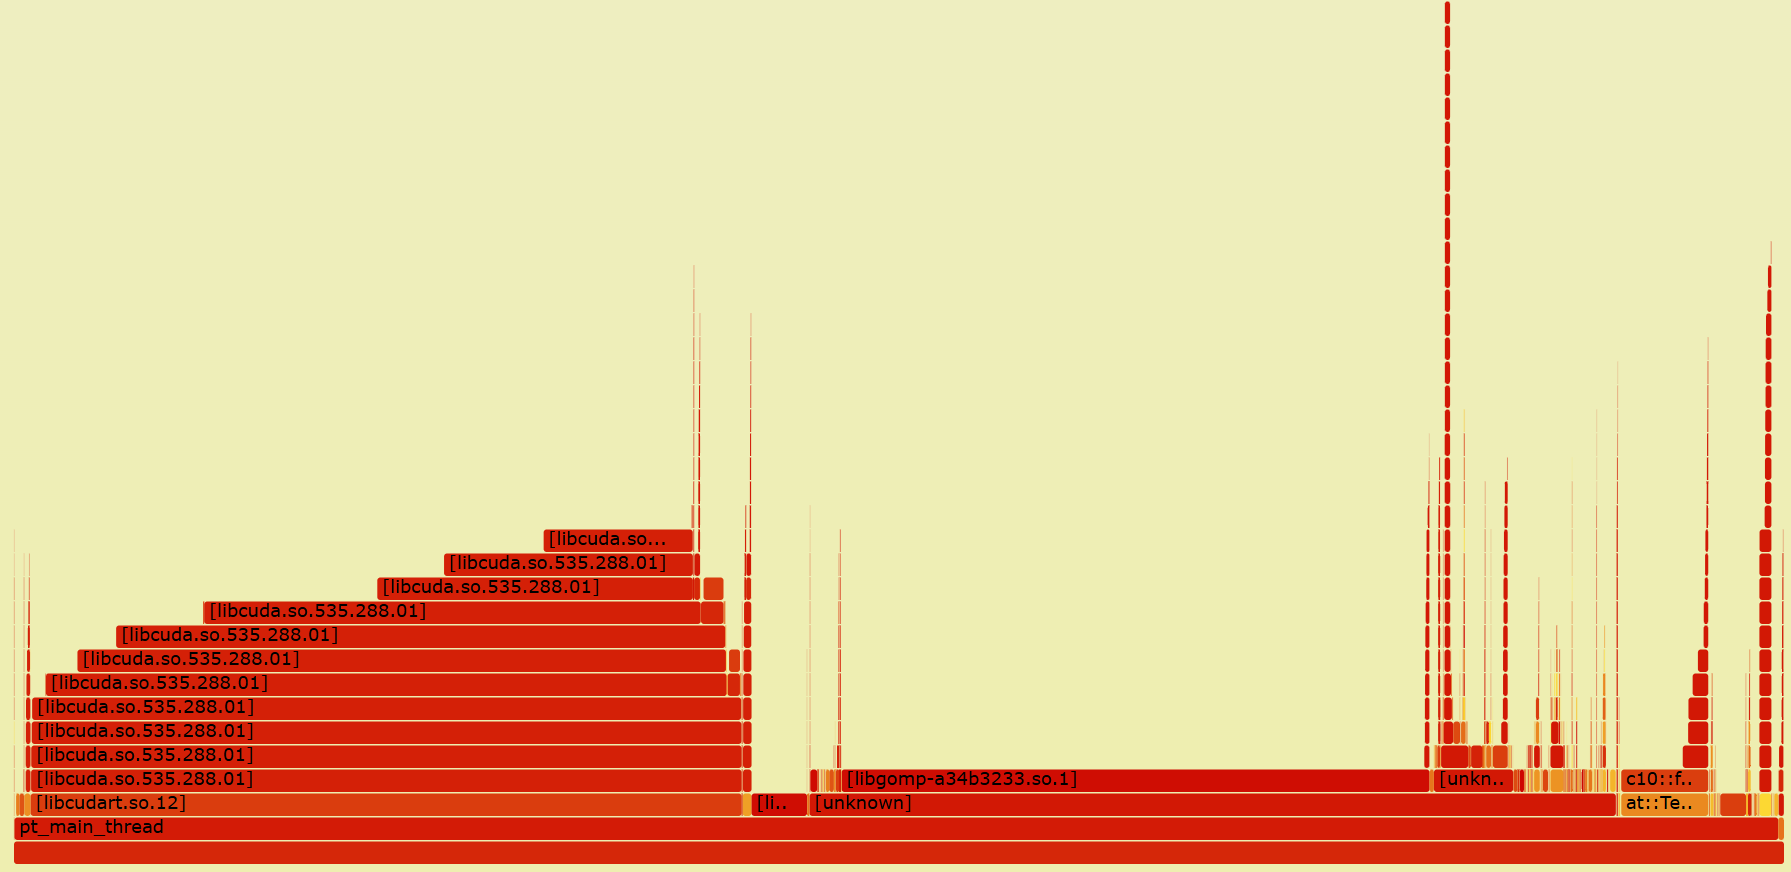
\includegraphics[width=0.8\textwidth]{flashGraphOfUT.png}
    \caption{Inference process flame graph}
    \label{fig:flashGraph_ut}
\end{figure}

From the perspective of flame graph analysis, the left side exhibits a broad horizontal cascade (layers of \textbf{libcuda.so}) while the right side shows dense, fine-grained vertical stacks (scheduling traces of \textbf{c10::} and \textbf{at::}), reflecting significant operator fragmentation and kernel launch overhead. This indicates that the system is in a typical CPU-bound state: numerous small, discrete memory-bound operations frequently interrupt the GPU execution pipeline, causing the CPU to spend more time on low-level driver API calls and context switches than the actual computation on CUDA cores.

Implementing fine-grained operator fusion can reconstruct the spatio-temporal locality of data flow. By explicitly rewriting frequently occurring composite operator blocks (such as normalization and activation functions) into a single kernel, repeated read-write operations of intermediate activations to GPU HBM can be eliminated. This keeps data circulation closed within low-latency SRAM, thereby accelerating model inference optimization.

\subsubsection{Multi-GPUs}
\

In the practical implementation of model inference, the process consists of n iterations, as specified by the n\_iter parameter in the run\_world\_model\_interaction.sh script. Each iteration can be further divided into two sequential stages: first, the VLA model generates an action sequence; second, the world model takes this action sequence as input and produces corresponding frames. The output of each iteration serves as the input for the next, making the inference process of unifolm-wma inherently sequential.

However, with respect to the attention computations involved in different parts of the denoising process, an optimization can be envisioned for a dual-GPU setup. Specifically, the initialization data required for model inference is simultaneously loaded into both GPUs. One implementation approach involves the CPU first reading the data from an SSD into memory, then transferring it to the GPU local to the CPU, after which this GPU copies the data to the other GPU. Subsequently, both GPUs perform denoising in parallel, each handling their respective portion of the attention computation. The computed attention results are then distributed across GPUs via blocking operations to facilitate subsequent steps, thereby enabling parallel processing of the attention computation workload.
% \ 
%模型并行、流水线并行等方法。


\subsection{Conclusion}
\

In the optimization of UnifoLM-WMA inference, our team systematically evaluated several strategies, including single-node NUMA affinity, mixed-precision arithmetic, I/O enhancements, FlashAttention, and DeepCache. To maximize inference throughput while strictly adhering to the mandated fidelity threshold ($PSNR > 25 dB$), we adopted a balanced trade-off approach. Our final deployment integrates mixed-precision, I/O optimizations, and FlashAttention; however, the DeepCache strategy was excluded to preserve baseline quality, and operator fusion remains in the exploratory phase. Under this configuration, the system achieved a mean acceleration ratio of 1.426$\times$. Moving forward, we intend to further refine and synergistically combine diverse optimization methodologies tailored to the specific algorithmic architecture, aiming to enhance inference efficiency while ensuring full PSNR compliance.


\clearpage